
\documentclass[10pt]{article}

\usepackage{graphicx,amsmath,amssymb,subfigure,enumerate,versions}
\usepackage{multicol,multirow,mdframed}
\usepackage{epstopdf}
\usepackage{pstricks,auto-pst-pdf}
\usepackage{pst-all}
\usepackage{pst-ode}
\usepackage{pst-math}
\DeclareGraphicsExtensions{.png,.jpg,.pdf}

% ************ Page Margins *************
\hoffset=-1.3in
\setlength{\textwidth}{7.5in}
%%%%% MARGINS
\topmargin 0pt
\advance \topmargin by -\headheight
\advance \topmargin by -\headsep
\textheight 9.5in

% ************ Shortcuts *************
\newcommand{\Z}{\mbox{\sf Z\hspace{-1.5mm}Z}}
\newcommand{\SolutionSeparator}{ \hfill \hfill \hrule \hfill \hfill }
\newcommand{\R}{\mbox{\rm I\hspace{-0.75mm}R}}
\columnsep=0.75in
\newcommand{\vsc}{\vspace{1mm}}
\newcommand{\D}{\Delta }
\newcommand{\ifd}{f(x)~dx}
\newcommand{\dd}{\frac{dy}{dx} \,} 
\newcommand{\der}[2]{\frac{d{#1}}{d{#2}} \,}
\newcommand{\ddx}[1]{\frac{d {#1}}{dx} \,} 
\newcommand{\ddy}[1]{\frac{d {#1}}{dy} \,} 
\newcommand{\ddz}[1]{\frac{d {#1}}{dz} \,} 
\newcommand{\ddt}[1]{\frac{d {#1}}{dt} \,} 
\newcommand{\ds}{\displaystyle } 
\newcommand{\la}{\lambda } 
\newcommand{\del}{\nabla } 
\newcommand{\zx}{\frac{\partial z}{\partial x} \,}
\newcommand{\zy}{\frac{\partial z}{\partial y} \,}
\newcommand{\dx}{\frac{\partial f}{\partial x} \,}
\newcommand{\dy}{\frac{\partial f}{\partial y} \,}
\newcommand{\pp}[2]{\frac{\partial {#1}}{\partial {#2}} \,}
\newcommand{\ppx}{\frac{\partial }{\partial x} \,}
\newcommand{\ppy}{\frac{\partial }{\partial y} \,}
\renewcommand{\thesection}{\Roman{section}}
\newcommand{\vi}{\vec{i}}
\newcommand{\vj}{\vec{j}}
\newcommand{\vk}{\vec{k}}
\newcommand{\vv}{\vec{v}}
\newcommand{\lan}{\left\langle}
\newcommand{\ran}{\right\rangle}
\newcommand{\degr}{^{\circ}}

% *** Define the printed question style ***
\newcommand{\q}[1]{ {\em #1} }
% \renewcommand{\q}[1]{ {} }

\newcommand{\notice}{ \begin{center}Some problems and solutions
    selected or adapted from \\ Stewart {\em Calculus-Early
      Transcendentals} and Hughes-Hallett {\em Calculus} .\end{center}
}

% *** Overwrite, if desired, the question format
\input{DocumentFormat.tex}

% *** Footnoting with symbols ***
\long\def\symbolfootnote[#1]#2{\begingroup%
\def\thefootnote{\fnsymbol{footnote}}\footnote[#1]{#2}\endgroup}

\newcommand{\WeekTitleOne}{Derivatives - Foundations}
\newcommand{\WeekTitleTwo}{Derivatives - Linearization and Applications}
\newcommand{\WeekTitleThree}{Derivatives - Applications}
\newcommand{\WeekTitleFour}{Integrals - Foundations}
\newcommand{\WeekTitleFive}{Integrals - Techniques}
\newcommand{\WeekTitleSix}{Integrals - Modeling}
\newcommand{\WeekTitleSeven}{Differential Equations - }
\newcommand{\WeekTitleEight}{Differential Equations - }
\newcommand{\WeekTitleNine}{Differential Equations - }
\newcommand{\WeekTitleTen}{Linear Algebra - }
\newcommand{\WeekTitleEleven}{Linear Algebra - }
\newcommand{\WeekTitleTwelve}{Linear Algebra - }


\begin{document}


\begin{center}
\subsection*{MNTC P01 - Week \#4 - \WeekTitleFour}
\end{center}

\begin{enumerate}[1.]
\subsection*{Distance And Velocity}

\begin{multicols}{2}
%*****************
\item
  \begin{Question}
    The graph below shows the velocity, $v$, of an object (in
    meters/sec). Estimate the total distance the object traveled
    between $t = 0$ and $t = 6$.

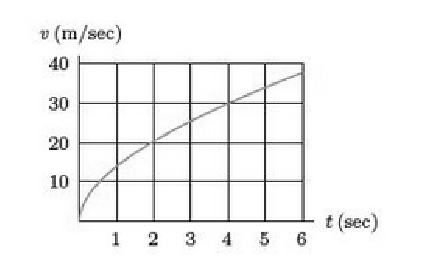
\includegraphics[width=0.7\linewidth]{graphics/Week04_DistanceAndVelocity/Velocity_1}
    
  \end{Question}
  \begin{Solution}
    Just counting the squares (each of which has area representing 10
    (m/s)$\cdot$(s) = 10 m of distance), and allowing for the partial
    squares, we can see that the area under the curve from $t=0$ to
    $t=6$ is between 140 and 150 units.  Therefore the distance
    traveled is between 140 and 150 meters.
  \end{Solution}

%*****************
\item
  \begin{Question}
    The figure below shows the velocity of a particle, in cm/sec,
    along the $t$-axis for $-3 \le t \le 3$ ($t$ in seconds). 
    \begin{enumerate}
    \item Describe the motion in words. Is the particle changing
      direction or always moving in the same direction? Is the
      particle speeding up or slowing down?
    \item Make over- and underestimates of the distance traveled for 
      $-3 \le t \le 3$.
    \end{enumerate}

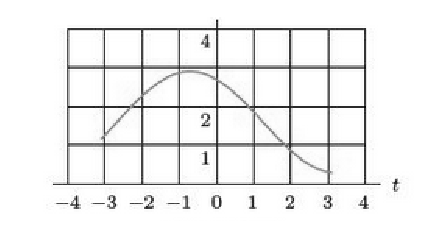
\includegraphics[width=0.7\linewidth]{graphics/Week04_DistanceAndVelocity/Velocity_2}
  \end{Question}
  \begin{Solution}
    \begin{enumerate}[(a)]
    \item The velocity is always positive, so the particle is moving
      in the same direction throughout.  However, the particle is
      speeding up until shortly before $t=0$, and slowing down
      thereafter.
    \item The distance traveled is represented by the area under the
      curve.  Using whole grid squares, we can overestimate the area
      as 3+3+3+3+2+1 = 15 squares, and we can underestimate the area
      as 1+2+2+1+0+0= 6 squares.  Each square represents 1
      (cm/sec)$\cdot$(s) = 1 cm, so the particle moved in one
      direction between 6 and 15 cm.

    \end{enumerate}
    
  \end{Solution}

%*****************
\item
  \begin{Question}
    Consider the following table of values for $f(t)$.
\begin{center}
\begin{tabular}{|c|c|c|c|c|c|} \hline
$t$&15&17&19&21&23\\ \hline
$f(t)$& 10&13&18&20&30 \\ \hline
\end{tabular}
\end{center}
\begin{enumerate}[(a)]
\item If we divide the time interval into $n = 4$ sub-intervals, what is $\Delta t$? What are $t_0, t_1, t_2, t_3, t_4$? What are $f(t_0), f(t_1), f(t_2), f(t_3), f(t_4)$? 
\item Find the left and right sums using $n = 4$. 
\item If we divide the time interval into $n = 2$ sub-intervals, what is $\Delta t$? What are $t_0, t_1, t_2$? What
  are $f(t_0), f(t_1), f(t_2)$?
\item Find the left and right sums using $n = 2$. 
\end{enumerate}
    
  \end{Question}
  \begin{Solution}
    \begin{enumerate}[(a)]
    \item With $n=4$, we have $\Delta t = 2$.  Then \\
$t_0 = 15, t_1 = 17, t_2 = 19, t_3 = 21, t_4 =23$, \\
and \\
$f(t_0) = 10, f(t_1) = 13, f(t_2) = 18, f(t_3) = 20, f(t_4) = 30$. \\
\item \begin{align*}
\mbox{Left sum} &= (10)(2) + (13)(2) + (18)(2) + (20)(2) & \\
&= 122 \\
\mbox{Right sum} &= (13)(2) + (18)(2) + (20)(2) + (30)(2) \\
&= 162 \\
\end{align*}
\item  With $n = 2$,we have $\Delta t = 4$. Then \\
$t_0 = 15; t_1 = 19; t_2 = 23$ and \\
$f(t_0) = 10; f(t_1) = 18; f(t_2) = 30$.
\item
  \begin{align*}
\mbox{Left sum} = (10)(4) + (18)(4) = 112 \\
\mbox{Right sum} = (18)(4) + (30)(4) = 192 \\
  \end{align*}
    \end{enumerate}
  \end{Solution}

%*****************
\item
  \begin{Question}
    Consider the following table of values for $f(t)$.
\begin{center}
\begin{tabular}{|c|c|c|c|c|c|} \hline
$t$&0&4&8&12&16\\ \hline
$f(t)$&25&23&22&20&17 \\ \hline
\end{tabular}
\end{center}
    \begin{enumerate}[(a)]
    \item If we divide the time interval into $n = 4$ subintervals,
      what is $\Delta t$? What are $t_0, t_1, t_2, t_3, t_4$? What are
      $f(t_0), f(t_1), f(t_2), f(t_3), f(t_4)$?
    \item Find the left and right sums using $n = 4$.
    \item If we divide the time interval into $n = 2$ subintervals,
      what is $\Delta t$? What are $t_0, t_1, t_2$? What are $f(t_0),
      f(t_1), f(t_2)$?
    \item Find the left and right sums using $n = 2$.
    \end{enumerate}
  \end{Question}
  \begin{Solution}
    \begin{enumerate}[(a)]
    \item With $n = 4$, we have $\Delta t$ = 4. Then \\
$t_0 = 0; t_1 = 4; t_2 = 8; t_3 = 12; t_4 = 16$ and  \\
$f(t_0) = 25; f(t_1) = 23; f(t_2) = 22; f(t_3) = 20; f(t_4) = 17$
\item
\begin{align*}
\mbox{Left sum} & = (25)(4) + (23)(4) + (22)(4) + (20)(4) \\
& = 360 \\
\mbox{Right sum} & = (23)(4) + (22)(4) + (20)(4) + (17)(4) \\
& = 328 \\
\end{align*}
\item  With $n = 2$,we have $\Delta t = 8$. Then\\
$t_0 = 0; t_1 = 8; t_2 = 16$ and $f(t_0) = 25; f(t_1) = 22; f(t_2) = 17$
\item 
\begin{align*}
\mbox{Left sum} & = (25)(8) + (22)(8) = 376\\
\mbox{Right sum} & = (22)(8) + (17)(8) = 312 \\
\end{align*}
    \end{enumerate}
  \end{Solution}

%*****************
\item
  \begin{Question}
    At time $t$, in seconds, your velocity, $v$, in meters/ second, is given by 
$$v(t) = 1+ t^2 \mbox{ for } 0 \le t \le 6.$$ Use $\Delta t = 2$ to estimate the distance traveled during this time. Find the upper and lower estimates, and then average the two.
\end{Question}

  \begin{Solution}
   Using $\Delta t = 2$,
   \begin{align*}
\mbox{Lower estimate} &= v(0) \cdot 2 + v(2) \cdot 2 + v(4) \cdot 2 \\
&= 1(2) + 5(2) + 17(2) \\
&= 46 \\
\mbox{Upper estimate} &= v(2) \cdot 2 + v(4) \cdot 2 + v(6) \cdot 2 \\
&= 5(2) + 17(2) + 37(2) \\
&= 118 \\
\mbox{Average} &= \frac{46+118}{2} \\
&= 82 \\
\mbox{Distance traveled} & \approx  82 \left(\frac{\mbox{m}}{\mbox{s}}\right) (\mbox{s}) = 82  \mbox{ meters.} 
   \end{align*}
  \end{Solution}

%*****************
\item
  \begin{Question}
    For time, $t$, in hours, $0 \le t \le 1$, a bug is crawling at a velocity, $v$, in meters/ hour given by 
$$v = \frac{1}{ 1 + t}.$$ Use $\Delta t$ = 0.2 to estimate the distance that the bug crawls during this hour. Find an overestimate and an underestimate. Then average the two to get a new estimate.
\end{Question}

  \begin{Solution}
    Using $\Delta t = 0.2$, our upper estimate is comes from using the
    smallest possible $t$ value on each interval, because that leads
    to the largest velocity.  I.e. we use $t_0 = 0$, $t_1 = 0.2$, etc.
\begin{align*}
\underbrace{\frac{1}{1 + 0}}_{v(t_0)} (0.2) +
\frac{1}{1 + 0.2} (0.2) +
\frac{1} {1 + 0.4} (0.2) \\ +
\frac{1}{1 + 0.6}(0.2) +
\frac{1}{1 + 0.8}
(0.2) \approx 0.75
\end{align*}
The lower estimate is
\begin{align*}
\frac{1} {1 + 0.2} (0.2) +
\frac{1} {1 + 0.4} (0.2) +
\frac{1} {1 + 0.6} (0.2) \\+
\frac{1} {1 + 0.8} (0.2) + 
\frac{1} {1 + 1} (0.2) \approx 0.65
\end{align*}
Since $v$ is a decreasing function, the bug has crawled more than 0.65
meters, but less than 0.75 meters. We average the two to get a better
estimate: 0.65 + 0.75 2 = 0.70 meters:
  \end{Solution}

%*****************
  \begin{Question}
For questions \ref{q:graph1_start} to \ref{q:graph1_end}, the graph
  shows the velocity, in cm/sec, of a particle moving along the
  $x$-axis. Compute the particle's change in position, left (negative)
  or right (positive), between times $t = 0$ and $t = 5$ seconds.
\end{Question}

\item ~\\\label{q:graph1_start} 
  \begin{Question}

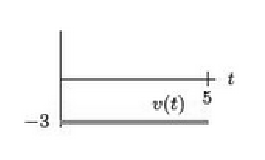
\includegraphics[width=0.4\linewidth]{graphics/Week04_DistanceAndVelocity/ParticleVelocity1}
  \end{Question}

  \begin{Solution}
    The velocity is constant and negative, so the change in position is $-3 \cdot 5$ cm, that is 15 cm to the left.
  \end{Solution}

%*****************
\item ~\\
  \begin{Question}
    
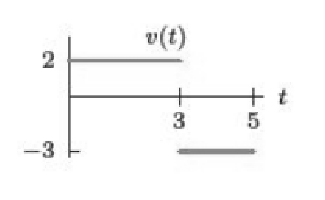
\includegraphics[width=0.4\linewidth]{graphics/Week04_DistanceAndVelocity/ParticleVelocity2}
  \end{Question}

  \begin{Solution}
    From $t = 0$ to $t = 3$, the velocity is constant and positive, so
    the change in position is $2 \cdot 3$ cm, that is 6 cm to the right. \\
    From $t = 3$ to $t = 5$, the velocity is negative and constant, so
    the
    change in position is $3 \cdot 2$ cm, that is 6 cm to the left.  \\
    Thus the total change in position is 0. The particle moves 6 cm to
    the right, followed by 6 cm to the left, and returns to where it
    started.
  \end{Solution}

%******************
\item ~ \\
  \begin{Question}
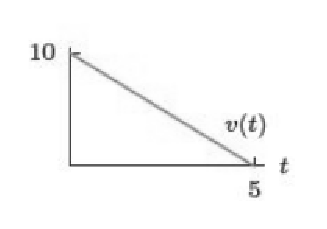
\includegraphics[width=0.4\linewidth]{graphics/Week04_DistanceAndVelocity/ParticleVelocity3}
  \end{Question}

  \begin{Solution}
    From $t = 0$ to $t = 5$ the velocity is positive so the change in
    position is to the right. The area under the velocity graph gives
    the distance traveled. The region is a triangle, and so has area
    $(1/2)bh = (1/2)5 \cdot 10 = 25$. Thus the change in position is 25 cm
    to the right.
  \end{Solution}

%******************
\item  ~ \\\label{q:graph1_end}
  \begin{Question}
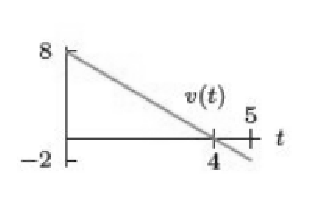
\includegraphics[width=0.4\linewidth]{graphics/Week04_DistanceAndVelocity/ParticleVelocity4}
  \end{Question}

  \begin{Solution}
    From $t = 0$ to $t = 4$ the velocity is positive so the change in
    position is to the right. The area under the velocity graph gives
    the distance traveled. The region is a triangle, and so has area
    $(1/2)bh = (1/2)4\cdot 8 = 16$. Thus the change in position is 16 cm
    to the right for$ t = 0$ to $t = 4$. 

    From $t = 4$ to $t = 5$, the velocity is negative so the change in
    position is to the left. The distance traveled to the left is
    given by the area of the triangle, $(1/2)bh = (1/2)1\cdot 2 =
    1$. 

    Thus the total change in position is $16-1= 15$ cm to the
    right.
  \end{Solution}

%*****************
\item
\begin{Question}
 A car going 80 ft/s ( about 90 km/h) brakes to a stop in five seconds. Assume the deceleration is constant. 
 \begin{enumerate}
 \item Graph the velocity against time, $t$, for $0 \le t \le 5$ seconds. 
 \item Represent, as an area on the graph, the total distance traveled
   from the time the brakes are applied until the car comes to a stop.
 \item Find this area and hence the distance traveled. 
% \item Now find the total distance traveled using antidifferentiation.
 \end{enumerate}
  \end{Question}

  \begin{Solution}
    \begin{enumerate}
    \item  ~\\
\includegraphics*[width=0.8\linewidth]{graphics/Week04_DistanceAndVelocity/graph_car_decel}
\item The total distance is represented by the shaded region $A$, the area under the graph of $v(t)$.
\item $A$ is a triangle, so its area is 
$$A = \frac{1}{2} \mbox{(base)(height)} = \frac{1}{2} (5 \mbox{ sec})(80 \mbox{ ft/s}) = 200 \mbox{ ft}$$
%\item 
    \end{enumerate}
    
  \end{Solution}


%******************
\item
  \begin{Question}
    A student is speeding down Route 11 in his fancy red Porsche when his radar system warns him of an obstacle 400 feet ahead. He immediately applies the brakes, starts to slow down, and spots a skunk in the road directly ahead of him. The ``black box'' in the Porsche records the car's speed every two seconds, producing the following table. The speed decreases throughout the 10 seconds it takes to stop, although not necessarily at a uniform rate. 
\begin{center}
\begin{tabular}{|l|r|r|r|r|r|r|} \hline
Time since &\multirow{2}{*}{0}&\multirow{2}{*}{2}&\multirow{2}{*}{4}&\multirow{2}{*}{6}&\multirow{2}{*}{8}&\multirow{2}{*}{10} \\ 
brakes applied &&&&&& \\ 
(sec) &&&&&& \\ \hline
Speed (ft/sec) &100&80&50&25&10&0  \\ \hline
\end{tabular}
\end{center}

    \begin{enumerate}[(a)]
\item What is your best estimate of the total distance the student's car traveled before coming to rest? 
\item Which one of the following statements can you justify from the information given? 
    \begin{enumerate}[(i)]
\item The car stopped before getting to the skunk. 
\item The ``black box'' data is inconclusive. The skunk may or may not have been hit. 
\item The skunk was hit by the car.
    \end{enumerate}
    \end{enumerate}
  \end{Question}

  \begin{Solution}
    To find the distance the car moved before stopping, we estimate
    the distance traveled for each two-second interval. Since speed
    decreases throughout, we know that the left-hand sum will be an
    overestimate to the distance traveled, and the right-hand sum an
    underestimate. Applying the formulas for these sums with $\Delta t
    = 2$ gives:
\begin{align*}
\mbox{LEFT} &= 2(100 + 80 + 50 + 25 + 10) = 530 \mbox{ ft} \\
\mbox{RIGHT} &= 2(80 + 50 + 25 + 10 + 0) = 330 \mbox{ ft}
\end{align*}
\begin{enumerate}[(a)]
\item The best estimate of the distance
    traveled will be the average of these two estimates, or 
    $\ds \frac{530 + 330}{2} = 430$ ft. 
\item  All we can be sure of is that the distance traveled lies between the upper and lower estimates
    calculated above. In other words, all the black-box data tells us
    for sure is that the car traveled between 330 and 530 feet before
    stopping.  So we can't be completely sure about whether it hit the
    skunk or not: answer (ii). 
\end{enumerate}
    
  \end{Solution}


%******************
\item
  \begin{Question}
     A baseball thrown directly upward at 96 ft/sec has velocity $v(t) = 96 - 32t$ ft/ sec at time $t$ seconds.
     \begin{enumerate}[(a)]
\item Graph the velocity from $t = 0$ to $t = 6$. 
\item When does the baseball reach the peak of its flight? How high does it go? 
\item How high is the baseball at time $t = 5$?
     \end{enumerate}
  \end{Question}
  \begin{Solution}
    \begin{enumerate}[(a)]
    \item  See the figure below.

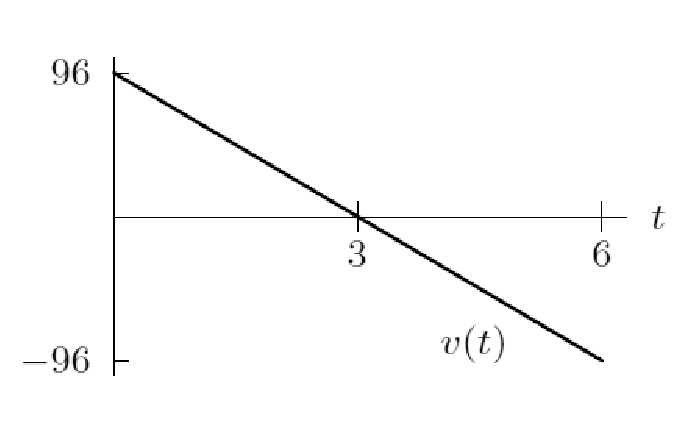
\includegraphics[width=0.7\linewidth]{graphics/Week04_DistanceAndVelocity/ChangeInPosition_2}

\item The peak of the flight is when the velocity is 0, namely $t =
  3$. The height at $t = 3$ is given by the area under the graph of
  the velocity from $t = 0$ to $t = 3$; see the figure above. The
  region is a triangle of base 3 seconds and altitude 96 ft/sec, so
  the height is $(1/2)3 \cdot 96 = 144$ feet.
\item The velocity is negative from $t = 3$ to $t = 5$, so the motion
  is downward then. The distance traveled downward can be calculated
  by the area of the triangular region which has base of 2 seconds and
  altitude of -64 ft/sec. Thus, the baseball travels $(1/2)2 \cdot 64
  = 64$ feet downward from its peak height of 144 feet at $t =
  3$. Thus, the height at time $t = 5$ is the total change in
  position, $144 - 64 = 80$ feet.
    \end{enumerate}
  \end{Solution}

%******************
\item
  \begin{Question}
    Two cars start at the same time and travel in the same direction
    along a straight road. The graph below gives the velocity, $v$, of
    each car as a function of time, $t$. Which car:
  \begin{enumerate}[(a)]
  \item Attains the larger maximum velocity? 
  \item Stops first? 
  \item Travels farther?
  \end{enumerate}
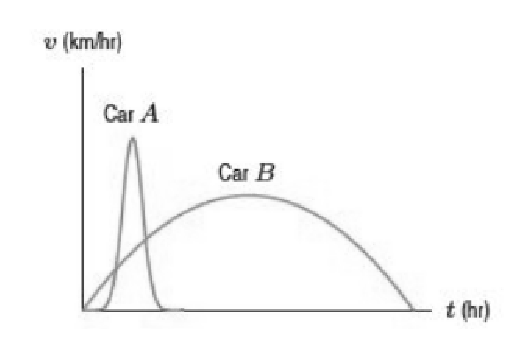
\includegraphics[width=0.7\linewidth]{graphics/Week04_DistanceAndVelocity/CarVelocity1}
  \end{Question}

  \begin{Solution}
    \begin{enumerate}[(a)]
    \item Car A has the largest maximum velocity because the peak of
      car A's velocity curve is higher than the peak of B's.
    \item Car A stops first because the curve representing its
      velocity hits zero (on the $t$-axis) first.
    \item Car B travels farther because the {\bf area} under car B's
      velocity curve is the larger, and area under the velocity graph
      reprsents distance.
    \end{enumerate}
  \end{Solution}

%******************
\item
  \begin{Question}
    Two cars travel in the same direction along a straight road. The graph below shows the velocity, $v$, of each car at time $t$. Car B starts 2 hours after car A and car B reaches a maximum velocity of 50 km/ hr. 
    \begin{enumerate}[(a)]
    \item For approximately how long does each car travel? \item
      Estimate car A's maximum velocity. \item Approximately how far
      does each car travel?
    \end{enumerate}
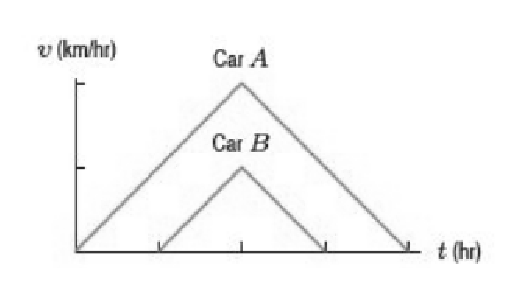
\includegraphics[width=0.7\linewidth]{graphics/Week04_DistanceAndVelocity/CarVelocity2}
  \end{Question}

  \begin{Solution}
    \begin{enumerate}[(a)]
    \item Since car B starts at $t = 2$, the tick marks on the
      horizontal axis (which we assume are equally spaced) are 2 hours
      apart. Thus car B stops at $t = 6$ and travels for 4 hours.  Car
      A starts at $t = 0$ and stops at $t = 8$, so it travels for 8
      hours.
    \item Car A's maximum velocity is approximately twice that of car B (50 km/h), so A's max velocity is 100 km/hr.
    \item The distance traveled is given by the area of under the
      velocity graph. Using the formula for the area of a triangle,
      the distances are given by
\begin{align*}
\mbox{Car A travels} &=
\frac{1}{2} \cdot \mbox{Base }\cdot \mbox{Height} \\
& = \frac{1}{2} \cdot 8 \cdot 100 = 400 \mbox{ km} \\
\mbox{Car B travels} &=
\frac{1}{2} \cdot \mbox{Base }\cdot \mbox{Height}\\
& = \frac{1}{2} \cdot 4 \cdot 50 = 100 \mbox{ km}. \\
\end{align*}
    
    \end{enumerate}
  \end{Solution}

\end{multicols}
\hrulefill
\subsection*{The Definite Integral}

\begin{multicols}{2}
%*****************
\item
  \begin{Question}
    The figure below shows a Riemann sum approximation with $n$ subdivisions to $\ds \int_a^bf(x) dx$.
    \begin{enumerate}
    \item Is it a left- or right-hand approximation? Would the other one be larger or smaller? 
    \item What are $a$, $b$, $n$ and $\D x$?
    \end{enumerate}
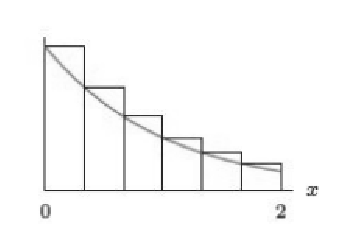
\includegraphics[width=0.4\linewidth]{graphics/Week04_TheDefiniteIntegral/DefiniteIntegral1}
  \end{Question}

  \begin{Solution}
    \begin{enumerate}[(a)]
    \item Left-hand sum. Right-hand sum would be smaller. 
    \item We have $a = 0$, $b = 2$, $n = 6$, $\Delta x = \frac{2}{6} = \frac{1}{3}$.
    \end{enumerate}
  \end{Solution}
%*****************
\item
  \begin{Question}
    Using the figure below, draw rectangles representing each of the
    following Riemann sums for the function $f$ on the interval $0 \le t \le
    8$. Calculate the value of each sum. 

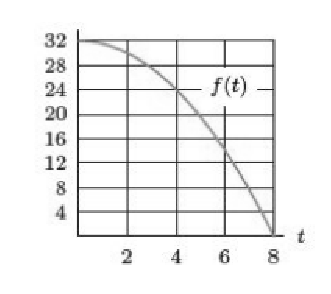
\includegraphics[width=0.5\linewidth]{graphics/Week04_TheDefiniteIntegral/DefiniteIntegral2}
\begin{enumerate}[(a)]
\item Left-hand sum with $\D t = 4.$
\item Right-hand sum with $\D t = 4.$
\item Left-hand sum with $\D t = 2$.
\item Right-hand sum with $\D t = 2.$
\end{enumerate}
  \end{Question}

  \begin{Solution}
\begin{tabular}{cc}
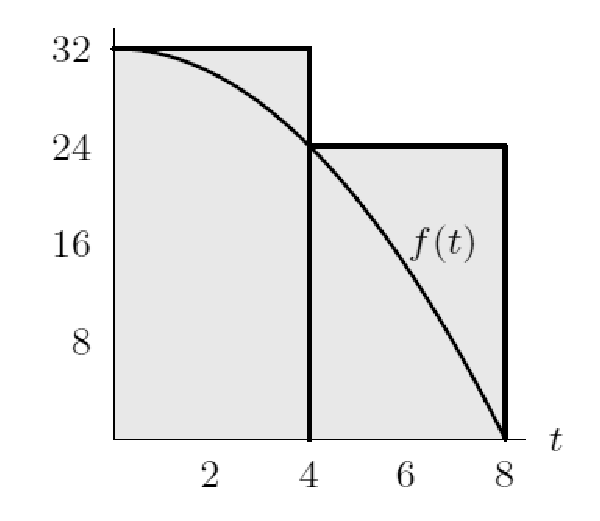
\includegraphics[width=0.4\linewidth]{graphics/Week04_TheDefiniteIntegral/DefiniteIntegral2_solutions1} & 
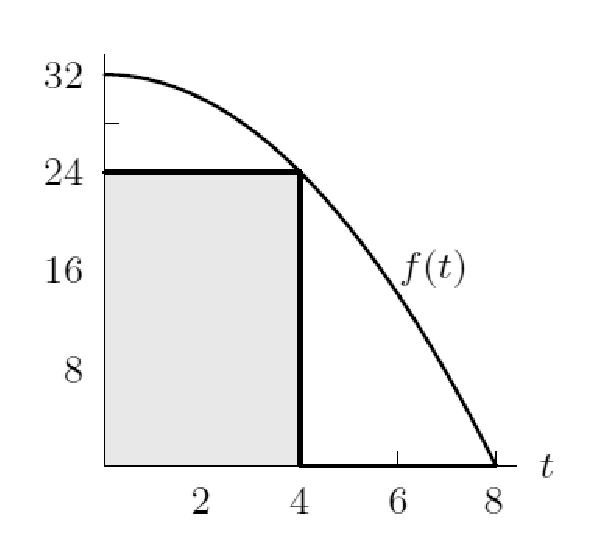
\includegraphics[width=0.4\linewidth]{graphics/Week04_TheDefiniteIntegral/DefiniteIntegral2_solutions2} \\
(a) & (b) \\ 
\end{tabular}

(a) The left-hand sum with $n=2$ intervals, or $\D t = 4$: $32 \cdot 4 + 24 \cdot 4$ = 224. \\
(b) The right-hand sum with $n=2$ intervals, or $\D t = 4$:  $24 \cdot 4 + 0 \cdot 4 = 96$.

\begin{tabular}{cc}
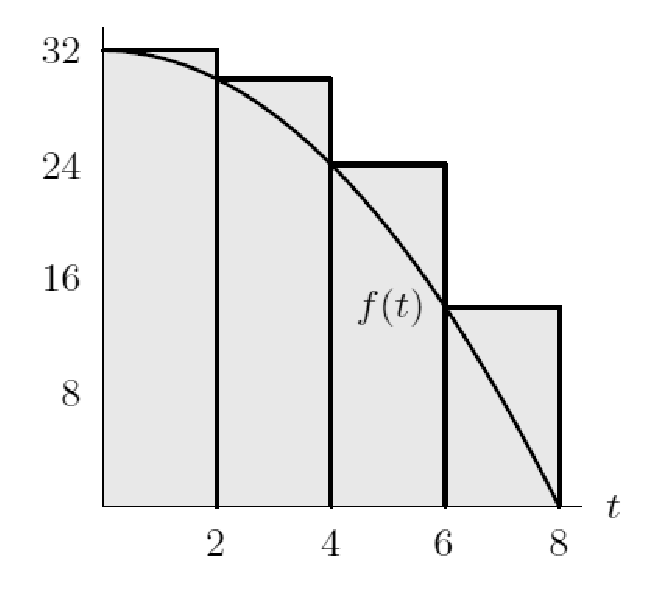
\includegraphics[width=0.4\linewidth]{graphics/Week04_TheDefiniteIntegral/DefiniteIntegral2_solutions3} & 
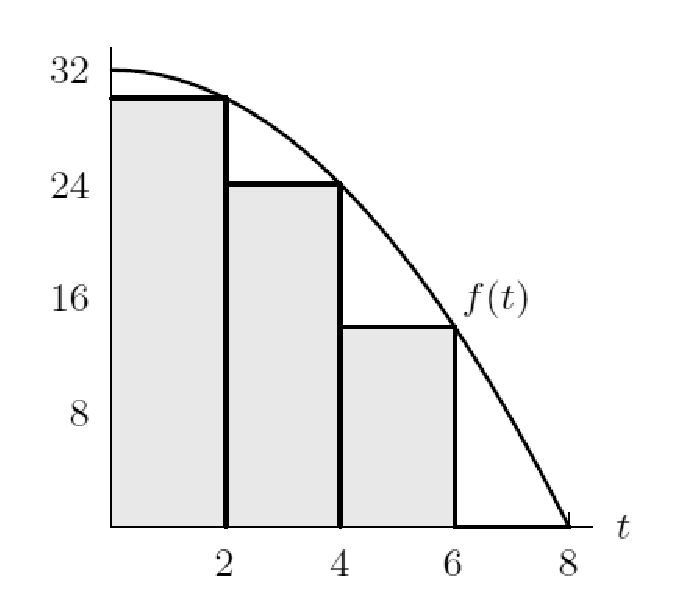
\includegraphics[width=0.4\linewidth]{graphics/Week04_TheDefiniteIntegral/DefiniteIntegral2_solutions4} \\
(c) & (d) \\ 
\end{tabular}

(c) Left-hand sum with $n=4$ intervals, or $\D t = 2$: $32 \cdot 2 + 30 \cdot 2 + 24 \cdot 2 + 14 \cdot 2 = 200$. \\
(d) Right-hand sum with $n=4$ intervals, or $\D t = 2$: $30 \cdot 2 + 24 \cdot 2 + 14 \cdot 2 + 0 \cdot 2 = 136$.


  \end{Solution}
%*****************
\item
  \begin{Question}
    The graph of a function $f(t)$ is given in the figure below.

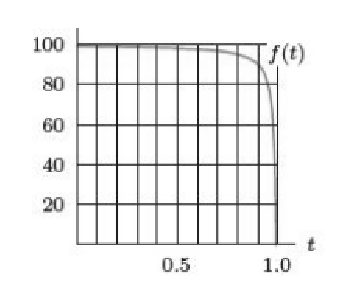
\includegraphics[width=0.6\linewidth]{graphics/Week04_TheDefiniteIntegral/DefiniteIntegral3}

Which of the following four numbers could be an estimate of $\ds \int_0^1f(t) ~dt$, accurate to two decimal places? Explain how you chose your answer.  \\
%\begin{tabular}{ll}
(a) -98.35   (b) 71.84 
(c) 100.12   (d) 93.47
%\end{tabular}
  \end{Question}

  \begin{Solution}
    The graph given shows that $f$ is positive for $0 \le t \le
    1$, so the integral value must be positive: the answer cannot be -98.35. 

    Since the graph is contained within a rectangle of height 100 and
    length 1, the answer 100.12 is too large.

    The graph of $f$ is well above the horizontal line y = 80 for
    $0\le t \le 0.95$, so the integral is likely much higher then
    71.84 $<$ 80, so out of the choices given the best estimate
    is 93.47: answer (d).
  \end{Solution}
%*****************
\item
  \begin{Question}
\begin{enumerate}[(a)]
\item What is the area between the graph of $f(x)$ shown below and
  the $x$-axis, between $x = 0$ and $x = 5$?
\item What is $\ds \int_0^5 f(x)~dx$?
\end{enumerate}
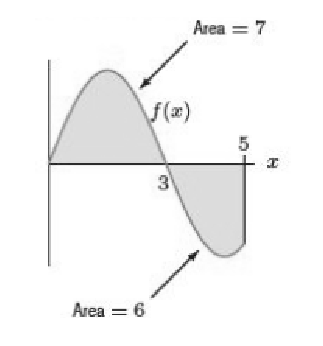
\includegraphics[width=0.6\linewidth]{graphics/Week04_TheDefiniteIntegral/DefiniteIntegral4}
  \end{Question}

  \begin{Solution}
    \begin{enumerate}[(a)]
    \item The total area between $f(x)$ and the $x$-axis is the sum of
      the two given areas, so area = 7 + 6 = 13.
\item  To find the integral, we note that from $x = 3$ to $x = 5$, the function lies below the $x$-axis, and hence makes a negative
contribution to the integral. So
$$\ds \int_0^5 f(x)~dx = \int_0^3 f(x)~dx + \int_3^5 f(x)dx = 7 - 6 = 1$$
    \end{enumerate}
  \end{Solution}
%*****************
\item
  \begin{Question}
    \begin{enumerate}[(a)]
    \item On a sketch of $y =\ln(x)$, represent the left Riemann sum with $n = 2$ approximating $\ds \int_1^2 \ln(x)~dx$. Write out the terms in the sum, but do not evaluate it. 
    \item On another sketch, represent the {\em right} Riemann sum with $n =
      2$ approximating $\ds \int_1^2 \ln(x)~dx$. Write out the terms in
      the sum, but do not evaluate it.
\item Which sum is an overestimate? Which sum is an underestimate?
    \end{enumerate}
  \end{Question}
  \begin{enumerate}[(a)]
  \item Below are the left and right sums respectively. \\
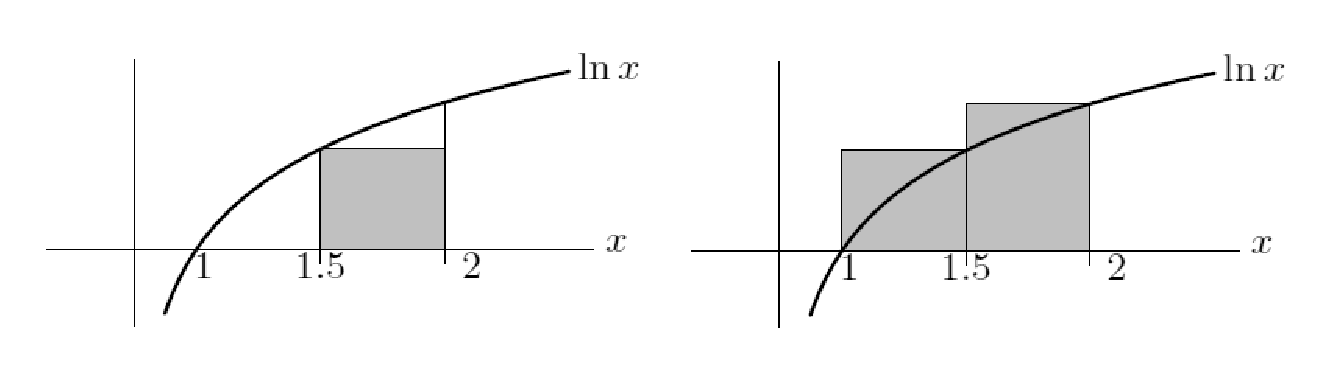
\includegraphics[width=0.9\linewidth]{graphics/Week04_TheDefiniteIntegral/Ln_solutions} \\
\begin{align*}
\mbox{ Left sum} & = f(1) \Delta x + f(1.5) \Delta x  \\
& = \underbrace{(\ln1)}_{=0}0.5 + \ln(1.5)0.5 = (\ln 1.5)0.5
\end{align*}
\item \begin{align*}
\mbox{Right sum} & = f(1.5) \D x + f(2) \D x \\
& = (\ln1.5)0.5 + (\ln2)0.5 \\
\end{align*}
\item Right sum is an overestimate, left sum is an underestimate.
  \end{enumerate}
  \begin{Solution}
    
  \end{Solution}
%*****************
\item
  \begin{Question}
    Estimate $\ds \int_1^2 x^2~ dx$ using left- and right-hand sums
    with four subdivisions, and then averaging them. How far from the
    true value of the integral could your final estimate be?
  \end{Question}

  \begin{Solution}
 Left-hand sum gives: \\$1^2(1/4) + (1.25)^2(1/4) + (1.5)^2(1/4) + (1.75)^2(1/4) = 1.96875.$ 

Right-hand sum gives: \\$(1.25)^2(1/4) + (1.5)^2(1/4) + (1.75)^2(1/4) + (2)^2(1/4) = 2.71875$.

We improve our estimate the value of the integral by taking the
average of these two sums, which is 2.34375.

Since $x^2$ is always increasing on $1 \le x \le 2$, the true value
of the integral lies between 1.96875 and 2.71875. Thus the most our
estimate could be off is 0.375 (half of the range from 2.34 to the
lower and upper bounds 1.97 and 2.72). We expect our 2.34 estimate to
be much closer than that possible error bound though. (And it is: the
true value of the integral is $7/3 \approx 2.333$.)
  \end{Solution}
%*****************
\item
  \begin{Question}
    Without computing the sums, find the difference between the right-
    and left-hand Riemann sums if we use $n = 500$ subintervals to
    approximate $\ds \int_{-1}^1(2x^3 + 4)~dx$.
  \end{Question}

  \begin{Solution}
    We have $\D x = 2/500 = 1/250$. The formulas for the left- and right-hand Riemann sums give us that
\begin{align*}
\mbox{Left} &= \D x[f(-1) + f(-1 + \D x) + \ldots \\
& + f(1 - 2\D x) + f(1 - \D x)] \\
\mbox{Right} & = \D x[f(-1 + \D x) + f(-1 + 2\D x) + \ldots \\
& + f(1 - \D x) + f(1)]:
\end{align*}
 Subtracting these yields
\begin{align*}
\mbox{Right - Left} & = \D x[f(1) - f(-1)] \\&=
\frac{1}{ 250} [6 - 2] =
\frac{4}{250}
= \frac{2}{ 125}.
\end{align*}
The estimates from the Right and Left sums will differ by 2/125.
  \end{Solution}
%*****************
\item
  \begin{Question}
    Without computation, decide if $\ds \int_0^{2\pi} e^{-x} \sin
    x~dx$ is positive or negative. [Hint: Sketch $e^{-x} \sin(x)$].
  \end{Question}

  \begin{Solution}

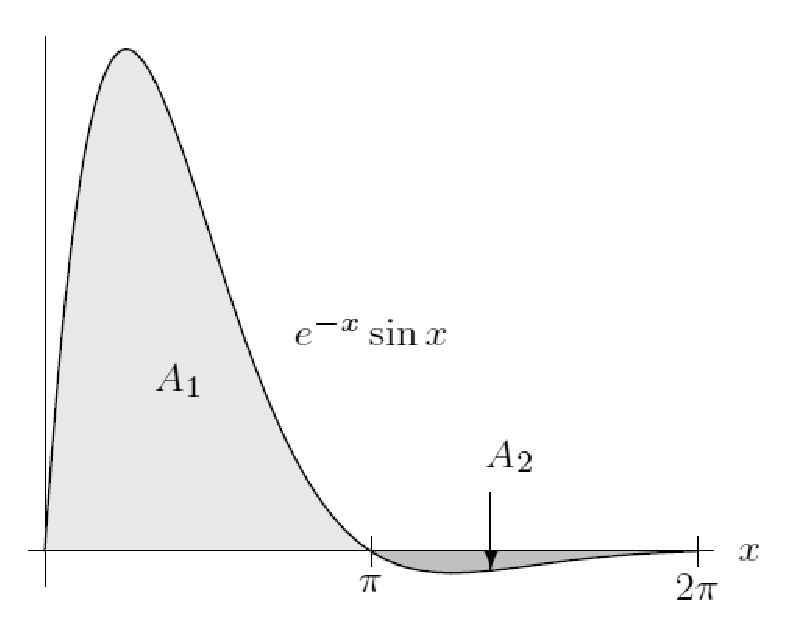
\includegraphics[width=0.6\linewidth]{graphics/Week04_TheDefiniteIntegral/ExpSin_solutions} \\

Looking at the graph of $y = e^{-x} \sin x$ shown above (remember the
sketching of variable amplitudes earlier in the course!), for $0 \le x
\le 2\pi$, we see that the area, $A_1$, which contributes a positive
amount to the integral $\ds \int_0^{2 \pi} e^{-x} \sin(x)~dx$, is much
larger than the area $A_2$, which contributes a negative amount to the
integral.

Since the positive integral contributions are larger than the negative, the overall integral will be positive. 
  \end{Solution}
%*****************
\item
  \begin{Question}
    \begin{enumerate}[(a)]
    \item Graph $\ds f(x) = \begin{cases} 1-x & \text{ if $0 \le x\le 1$}  \\
x-1 & \text{ if $1 < x\le 2$}  \\
\end{cases}$
\item Find the {\em exact} value of $\ds \int_0^2 f(x)~ dx$ (hint: sketch and see what shapes you get). 
\item Calculate the 4-term left Riemann sum approximation to the
  definite integral. How does the approximation compare to the exact
  value?
    \end{enumerate}
  \end{Question}

  \begin{Solution}
    \begin{enumerate}[(a)]
    \item  ~\\
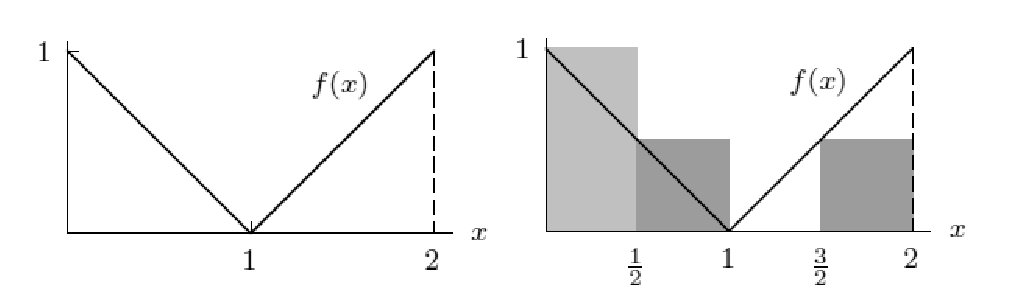
\includegraphics[width=0.9\linewidth]{graphics/Week04_TheDefiniteIntegral/Piecewise_solutions} \\ 
\item The area is made up of two triangles, with total area of 2 $\times$ (1/2)(1)(1) = 1 square unit. 
\item Using $\D x = 1/2$ in the 4-term Riemann sum shown in right-side
  graph above, we have 
\begin{align*}
& \mbox{Left hand sum}  \\
&= f(0)\D x + f(0.5)\D x + f(1)\D x + f(1.5)\D x \\
& = 1 \left(\frac{1}{2} \right) + \frac{1}{2} \left(\frac{1}{2} \right) + 0 \left(\frac{1}{2} \right) + \frac{1}{2} \left(\frac{1}{2} \right) \\
&  = 1.
\end{align*} We notice that in this case the approximation is exactly
equal to the exact value of the integral.  This is mostly coincidence
due to the simple shape of $f(x)$.  In general, approximations will
not work out to be exactly the same as the value of the integral.
    \end{enumerate}
  \end{Solution}
%*****************
\item
  \begin{Question}
Using the figure below, find the values of     

\begin{tabular}{ll}
(a) $\ds \int_a^b f(x)~dx$ & (b) $\ds  \int_b^c f(x)~dx$ \\
(c) $\ds \int_a^c f(x)~dx$ & (d) $\ds \int_a^c ~|f(x)|~dx$
\end{tabular}

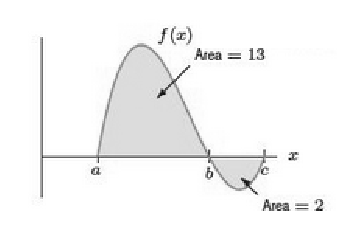
\includegraphics[width=0.6\linewidth]{graphics/Week04_TheDefiniteIntegral/DefiniteIntegral5}
  \end{Question}

  \begin{Solution}
    \begin{enumerate}[(a)]
    \item The area between the graph of $f(x)$ and the $x$-axis
      between $x = a$ and $x = b$ is 13, so $\ds \int_a^bf(x)~dx = 13$.
    \item Since the graph of $f(x)$ is below the x-axis for $b < x <
      c$, $\ds \int_b^c f(x)~ dx = -2$.
\item Since the graph of $f(x)$ is above the $x$-axis for $a < x < b$ and below for $b < x < c$,
$\ds \int_a^c f(x)~dx = 13 - 2 = 11$.
\item The graph of $|f(x)|$ is the same as the graph of $f(x)$, except
  that the part {\em below} the $x$-axis is reflected to be {\em
    above} it (see graph of $|f(x)|$ below).  Thus $\ds \int_a^c
  |f(x)|~ dx = 13 + 2 = 15$.

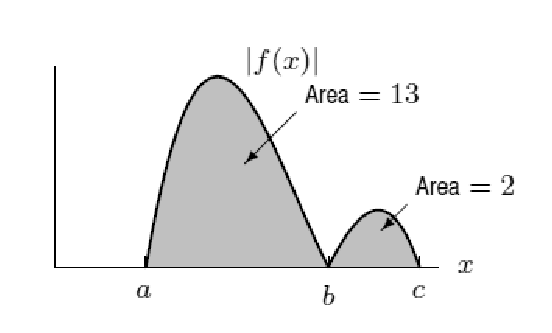
\includegraphics[width=0.6\linewidth]{graphics/Week04_TheDefiniteIntegral/AbsValue_solutions}
    \end{enumerate}
  \end{Solution}
%*****************
\item 
  \begin{Question}
    Given the figure below, and the statement that $\ds \int_{-2}^0 f(x)~dx = 4$, estimate 

\begin{tabular}{ll}
(a) $\ds \int_0^2 f(x)~dx$ & (b) $\ds  \int_{-2}^2 f(x)~dx$ \\
(c) The total shaded area.
\end{tabular}

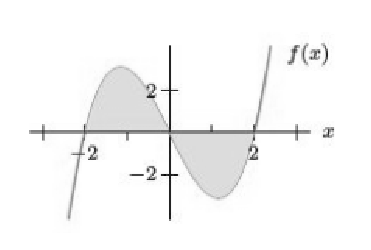
\includegraphics[width=0.6\linewidth]{graphics/Week04_TheDefiniteIntegral/DefiniteIntegral6}
  \end{Question}

  \begin{Solution}
    The region shaded between $x = 0$ and $x = 2$ appears to have
    approximately the same area as the region shaded between $x = -2$
    and $x = 0$, but it lies below the axis. Since $\ds \int_{-2}^0 f(x)~dx = 4$, we
    have the following results: 
    \begin{enumerate}
    \item $\ds \int_0^2f(x)~dx \approx  \mbox{ negative of }\int_{-2}^0 f(x)~dx =-4$
    \item  $\ds \int_{-2}^2 f(x)~ dx \approx 4 - 4 = 0$.  
    \item  The total area shaded is approximately 4 + 4 = 8.
    \end{enumerate}
  \end{Solution}
%*****************
\item
  \begin{Question}
    \begin{enumerate}[(a)]
    \item Using the graph below, find $\ds \int_{-3}^0 f(x)~dx$. 
\item If the area of the shaded region is $A$, estimate $\ds \int_{-3}^4 f(x)~ dx$.
    \end{enumerate}
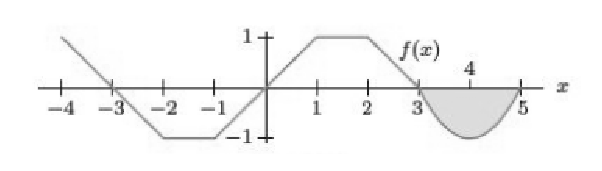
\includegraphics[width=0.9\linewidth]{graphics/Week04_TheDefiniteIntegral/DefiniteIntegral7}
  \end{Question}

  \begin{Solution}
    \begin{enumerate}
    \item $\ds \int_{-3}^0 f(x)~dx = -2$: counting squares or
      computing areas of the triangles and rectangles in this region.
    \item We break the integral over the interval $x=-3\ldots 5$ into
      pieces, each of which we can find the areas of.
\begin{align*}
 \int_{-3}^4 f(x)~dx & = \int_{-3}^0 f(x)~dx + \int_{0}^3 f(x)~dx + \int_{3}^4 f(x)~dx \\
& = -2 + 2 - \frac{A}{2} \\
&= \frac{-A}{2}
\end{align*}
    \end{enumerate}
  \end{Solution}
%*****************

\item
  \begin{Question}
Calculate the following approximations to $\ds \int_0^6 x^2~dx$.
     (a) LEFT(2); (b) RIGHT(2); \\(c) TRAP(2); (d) MID(2)
  \end{Question}

  \begin{Solution}
    \begin{enumerate}[(a)]
    \item Since two rectangles are being used, the width of each
      rectangle is $\D x = (6-0)/ 2 = 3$. The height is given by the
      left-hand endpoint so we have
\begin{align*}\mbox{LEFT}(2) & = f(0) \cdot 3 + f(3) \cdot 3   \\
& = 0^2 \cdot 3 + 3^2 \cdot 3 = 27 \\
\end{align*}
\item Again, $\D x = 3$. The height of each rectangle is given by the right-hand
  endpoint so we have
\begin{align*}
\mbox{RIGHT}(2) & = f(3) \cdot 3 + f(6) \cdot 3 \\
& = 32 \cdot 3 + 62 \cdot 3 = 135
\end{align*}
\item We know that TRAP is the average of LEFT and RIGHT and so
\begin{align*}
TRAP(2) = \frac{27 + 135}{ 2} = 81
\end{align*}
\item  $\D x = 3$ again. The height of each rectangle is given by the height at the midpoint so we have
  \begin{align*}
    MID(2) & = f(1.5) \cdot 3 + f(4.5) \cdot 3 \\
    & = (1.5)^2 \cdot 3 + (4.5)^2 \cdot 3 = 67.5
  \end{align*}
    \end{enumerate}
  \end{Solution}
%*****************
\item
  \begin{Question}
    \begin{enumerate}[(a)]
    \item Find LEFT(2) and RIGHT(2) for $\ds \int_0^4 (x^2 + 1)~ dx$. 
    \item Illustrate your answers to part (a) graphically. Is each
      approximation an underestimate or overestimate?
    \end{enumerate}
  \end{Question}

  \begin{Solution}
    \begin{enumerate}
\item  \begin{align*}
\mbox{LEFT(2)} & = 2 \cdot f(0) + 2 \cdot f(2) \\
& = 2 \cdot 1 + 2 \cdot 5 \\
&= 12 \\
\mbox{RIGHT(2)} & = 2 \cdot f(2) + 2 \cdot f(4) \\
&= 2 \cdot 5 + 2 \cdot 17 \\
&= 44   
\end{align*}
\item ~ \\ 
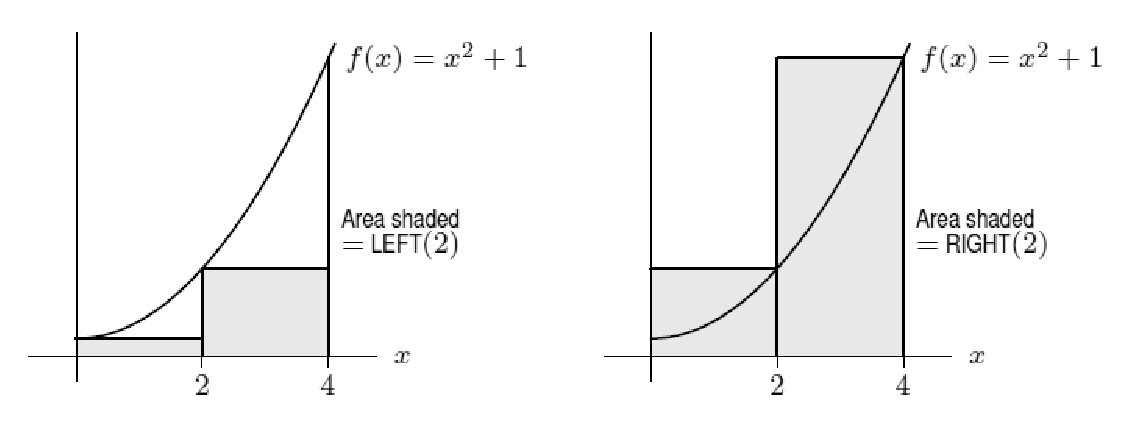
\includegraphics[width=0.9\linewidth]{graphics/Week04_TheDefiniteIntegral/Methods1_solutions1}

LEFT(2) will be an under-estimate, while RIGHT(2) will be an over-estimate. 
    \end{enumerate}
  \end{Solution}
%*****************
\item
  \begin{Question}
    \begin{enumerate}[(a)]
    \item Find MID(2) and TRAP(2) for $\ds \int_0^4 (x^2 + 1)~ dx$. 
    \item Illustrate your answers to part (a) graphically. Is each
      approximation an underestimate or overestimate?
    \end{enumerate}
  \end{Question}

  \begin{Solution}
    \begin{enumerate}
\item  \begin{align*}
\mbox{MID(2)} & = 2 \cdot f(1) + 2 \cdot f(3) \\
& = 2 \cdot 2 + 2 \cdot 10 \\
&= 24 \\
\mbox{TRAP(2)} & = \frac{\mbox{LEFT(2) + RIGHT(2)}}{2} \\
&= \frac{12 + 44}{2} \\
&= 28
\end{align*}
\item ~ \\ 
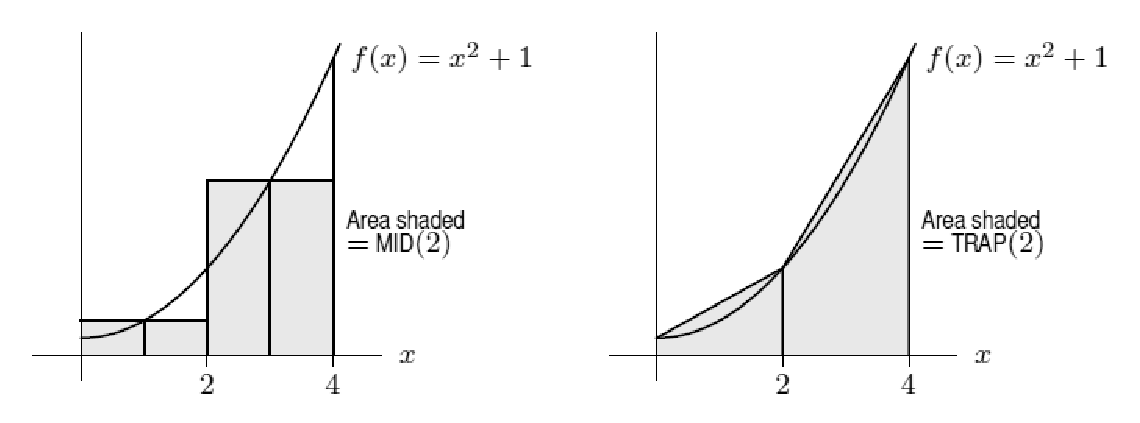
\includegraphics[width=0.9\linewidth]{graphics/Week04_TheDefiniteIntegral/Methods1_solutions2}
MID(2) is an underestimate, since $f(x) = x^2 + 1$ is concave up; this
means that the new growth of the function after the midpoint (missed
by MID) will be greater than extra area before (captured by MID).

Since $f(x)$ is concave up, TRAP(2) is an overestimate, because the
trapezoidal secant lines in the TRAP rule will always lie above the
original curve, leading to more area in the trapezoids than under the
curve.
    \end{enumerate}
  \end{Solution}
%*****************
\item
  \begin{Question}
   Calculate the following approximations to $\ds \int_0^{\pi} \sin(\theta) d\theta$. 
(a) LEFT(2); (b) RIGHT(2); \\
 (c) TRAP(2); (d) MID(2)   
  \end{Question}

  \begin{Solution}
    \begin{enumerate}
    \item Since two rectangles are being used, the width of each rectangle is $\D x = (\pi-0)/2 = \pi/2$. The height is given by the left-hand endpoint so we have
\begin{align*}
\mbox{LEFT}(2) & = f(0) \cdot \frac{\pi}{2}
+ f(\pi/2)  \cdot \frac{\pi}{2} \\
& = \sin 0  \cdot \frac{\pi}{2}
+ \sin(\pi/2)  \cdot \frac{\pi}{2} \\
& = \frac{\pi}{2} \\
\end{align*}

(b) Again $\D x = \pi/2$.  The height of each rectangle is given by
the right-hand endpoint so we have
\begin{align*}
RIGHT(2) & = f(\pi/2)  \cdot \frac{\pi}{2}
+ f(\pi)  \cdot \frac{\pi}{2} \\
& = \sin(\pi/2)  \cdot \frac{\pi}{2}
+ \sin(\pi)  \cdot \frac{\pi}{2} \\
& = \frac{\pi}{2}
\end{align*}
(c) We know that TRAP is the average of LEFT and RIGHT and so
\begin{align*}
\mbox{TRAP}(2) =\frac{\mbox{LEFT}(2) + \mbox{RIGHT}(2)}{2} = \frac{\pi/2 + \pi/2}{2} = \frac{\pi}{2}
\end{align*}
(d) Again, $\D x = \pi/2$.  The height of each rectangle is given by
the height at the midpoint so we have
\begin{align*}
\mbox{MID}(2) & = f(\pi/ 4)  \cdot \frac{\pi}{2}
+ f(3\pi/ 4)  \cdot \frac{\pi}{2} \\
&= \sin(\pi/4) \cdot \frac{\pi}{2}
+ \sin(3\pi/4)  \cdot \frac{\pi}{2} \\
&= \frac{\sqrt{2}\pi }{2}
\end{align*}
    \end{enumerate}
  \end{Solution}
%*****************
\item
  \begin{Question}
    Using the table below, estimate the total distance traveled from
    time $t = 0$ to time $t = 6$ using LEFT, RIGHT, and TRAP.
\begin{tabular}{lrrrrrrr} \hline
Time, $t$ (s) &0&1&2&3&4&5&6\\ \hline
 Velocity, $v$ (m/s)&3&4&5&4&7&8&11 \\ \hline
\end{tabular}
  \end{Question}

  \begin{Solution}
    Let $s(t)$ be the distance traveled at time $t$, and $v(t)$ be the velocity at time $t$. Then the distance traveled during the interval
$0 \le t \le 6$ is given by $\ds \int_0^6 v(t)~dt$.

We estimate the distance by estimating this integral.
From the table, we find: LEFT(6) = 31 m; RIGHT(6) = 39 m, TRAP(6) = 35 m.
  \end{Solution}
%*****************  

\begin{Question}
  For the functions in Problems \ref{q:choice_start} $-$
  \ref{q:choice_end}, pick which approximation- left, right,
  trapezoid, or midpoint- is guaranteed to give an {\em overestimate}
  for $\ds \int_0^5f(x) ~dx$, and which is guaranteed to give an {\em
    underestimate}. (There may be more than one.)
\end{Question}

\item ~\\ \label{q:choice_start}
  \begin{Question}
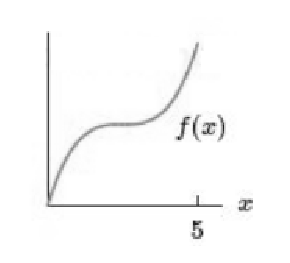
\includegraphics[width=0.4\linewidth]{graphics/Week04_TheDefiniteIntegral/Choice1}
    
  \end{Question}

  \begin{Solution}
$f(x)$ is increasing, so RIGHT gives an overestimate and LEFT gives an underestimate.
    
  \end{Solution}
%*****************
\item~ \\
  \begin{Question}
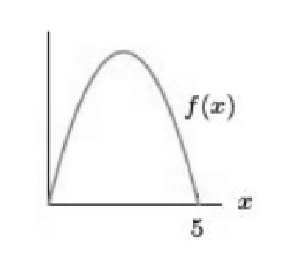
\includegraphics[width=0.4\linewidth]{graphics/Week04_TheDefiniteIntegral/Choice2}
    
  \end{Question}

  \begin{Solution}
$f(x)$ is concave down, so MID gives an overestimate and TRAP gives an underestimate.
    
  \end{Solution}
%*****************
\item~\\
  \begin{Question}
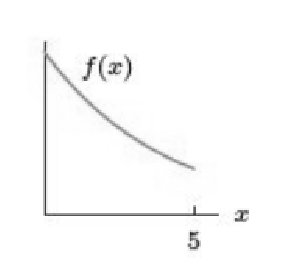
\includegraphics[width=0.4\linewidth]{graphics/Week04_TheDefiniteIntegral/Choice3}
    
  \end{Question}

  \begin{Solution}
$f(x)$ is decreasing and concave up, so LEFT and TRAP give overestimates and RIGHT and MID give underestimates.
    
  \end{Solution}
%*****************
\item~\\ \label{q:choice_end}
  \begin{Question}
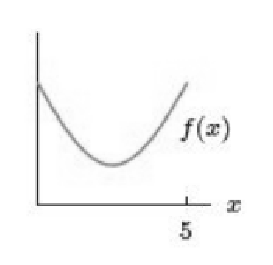
\includegraphics[width=0.4\linewidth]{graphics/Week04_TheDefiniteIntegral/Choice4}
    
  \end{Question}

  \begin{Solution}
$f(x)$ is concave up, so TRAP gives an overestimate and MID gives an underestimate.
    
  \end{Solution}
%*****************
%\item
%  \begin{Question}
%    \begin{enumerate}[(a)]
%    \item Values for $f(x)$ are in the table. Which of the four
%      approximation methods in this section is most likely to give the
%      best estimate of $\ds \int_0^{12} f( x)~ dx$? Estimate the
%      integral using this method.
%\item Assume $f(x)$ is continuous with no critical points or points of inflection on the interval $0 \le x \le 12$. Is the estimate found in part (a) an over- or underestimate? Explain. 
%
%\begin{tabular}{lrrrrr}\hline
%$x$& 0&3&6&9&12 \\ \hline
%$f(x)$&100&97&90&78&55    \\ \hline
%\end{tabular}
%    \end{enumerate}
%  \end{Question}
%
%  \begin{Solution}
%    
%  \end{Solution}
%*****************
\item
  \begin{Question}
    \begin{enumerate}[(a)]
    \item Find the exact value of $\ds \int_0^{2\pi} \sin \theta
      d\theta$ without calculation (i.e. from a sketch).
    \item Explain, using pictures, why the MID(1) and MID(2)
      approximations to this integral give the exact value.
    \item Does MID(3) give the exact value of this integral? How about
      MID($n$)? Explain.
    \end{enumerate}
  \end{Question}

  \begin{Solution}
    \begin{enumerate}[(a)]
    \item ~\\
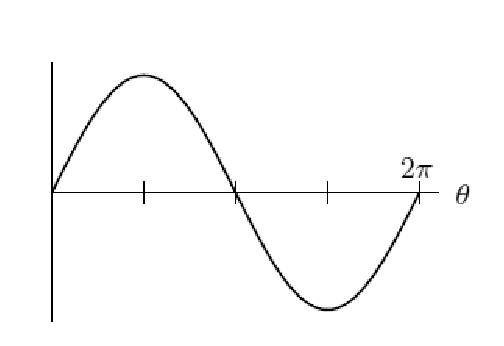
\includegraphics[width=0.6\linewidth]{graphics/Week04_TheDefiniteIntegral/Sine_solutions}

From the graph of sine above, and the fact that the integral includes
a complete $[0, 2\pi]$ cycle, it is clear from symmetry that the
positive and negative contributions to the integral must be equal, so
$$\int_0^{2 \pi} \sin(\theta)~d\theta = 0$$
\item Again, refer to the graph above. MID(1) is 0 since the midpoint of 0 and $2\pi$ is $\pi$ and $\sin \pi = 0$. Thus MID(1) = $2\pi \sin \pi = 0$.

The midpoints we use for MID(2) are $\pi/2$ and $3\pi/2$, and $\sin(\pi/2) = -\sin(3\pi/2)$. Thus MID(2) = $\pi \sin(\pi/2)+ \pi \sin(3\pi/2) = 0$.

\item MID(3) = 0. In general, MID($n$) = 0 for all $n$, even though
  your calculator (because of round-off error) might not return it as
  such. The reason is that $\sin(x) = -sin(2\pi - x)$. If we use
  MID($n$), we will always take sums where we are adding pairs of the
  form $\sin(x)$ and $\sin(2\pi- x)$, so the sum will cancel to 0. (If $n$ is
  odd, we will get a $\sin \pi$ in the sum which does not pair up with
  anything, but $\sin \pi$ is already 0.)
    \end{enumerate}
  \end{Solution}
%*****************
\item
  \begin{Question}
    The width, in feet, at various points along the fairway of a hole
    on a golf course is given in the figure below. If one pound of
    fertilizer covers 200 square feet, estimate the amount of
    fertilizer needed to fertilize the fairway.

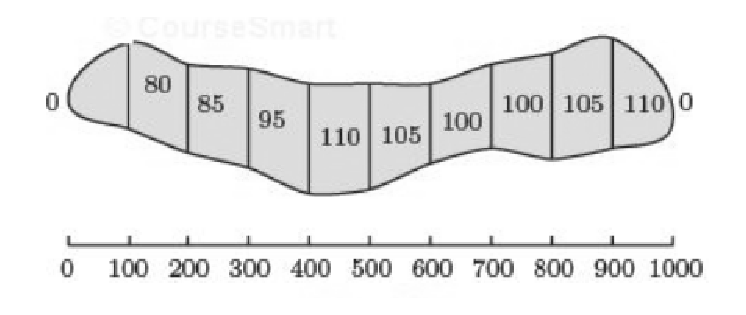
\includegraphics[width=0.9\linewidth]{graphics/Week04_TheDefiniteIntegral/GolfHole}
  \end{Question}

  \begin{Solution}
    We approximate the area of the playing field by using Riemann sums. From the data provided,
LEFT(10) = RIGHT(10) = TRAP(10) = 89,000 square feet.

Thus approximately
$\ds \frac{89,000 \mbox{ sq. ft.}}{200 \mbox{sq. ft./lb}} = 445$ lbs. of fertilizer
should be necessary.

Note that the fact that LEFT=RIGHT=TRAP doesn't mean there is no error
in the estimate; it actually means that the error is completely
unknown.  You will always have this relationship when the first and
last heights are equal because that makes LEFT = RIGHT, and then TRAP
(= average of LEFT and RIGHT) will equal the same value as well).
  \end{Solution}

\end{multicols}

\hrulefill

\subsection*{Definite Integrals in Modeling}

\begin{multicols}{2}
%*****************
\item
  \begin{Question}
    The rate at which the world's oil is being consumed is
    continuously increasing. Suppose the rate of oil consumption (in
    billions of barrels per year) is given by the function $r = f(t)$,
    where $t$ is measured in years and $t = 0$ is the start of 2004. 
    \begin{enumerate}[(a)]
    \item Write a definite integral which represents the total
      quantity of oil used between the start of 2004 and the start of
      2009.
    \item Suppose $r = 32e^{0.05t}$. Using a left-hand sum with five
    subdivisions, find an approximate value for the total quantity of
    oil used between the start of 2004 and the start of 2009. 
  \item Interpret each of the five terms in the sum from part (b) in
    terms of oil consumption.
    \end{enumerate}
  \end{Question}

  \begin{Solution}
    \begin{enumerate}[(a)]
    \item Quantity used = $\ds \int^5_0 f(t)~dt$.
\item Using a left sum, our approximation is
\begin{align*}&32e^{0.05(0)}+ 32e^{0.05(1)}+ 32e^{0.05(2)}+ 32e^{0.05(3)}+ 32e^{0.05(4)}  \\
&= 177.270.
\end{align*}
Since $f$ is an increasing function, the left endpoint values of $f$
are lower than anywhere else on the subintervals, so this represents
an underestimate.
\item Each term is a lower estimate of one year's consumption of oil. 
    \end{enumerate}
  \end{Solution}

%*****************
\item
  \begin{Question}
    As coal deposits are depleted, it becomes necessary to strip-mine
    larger areas for each ton of coal. The graph below shows the
    number of acres of land per million tons of coal that will be
    defaced during strip-mining as a function of the number of million
    tons removed, starting from the present day.
    \begin{enumerate}[(a)]
    \item Estimate the total number of acres defaced in extracting the
      next 4 million tons of coal (measured from the present
      day). Draw four rectangles under the curve, and compute their
      area.
    \item Re-estimate the number of acres defaced using rectangles
      above the curve.
    \item Combine your answers to parts (a) and (b) to get a better
      estimate of the actual number of acres defaced.
    \end{enumerate}
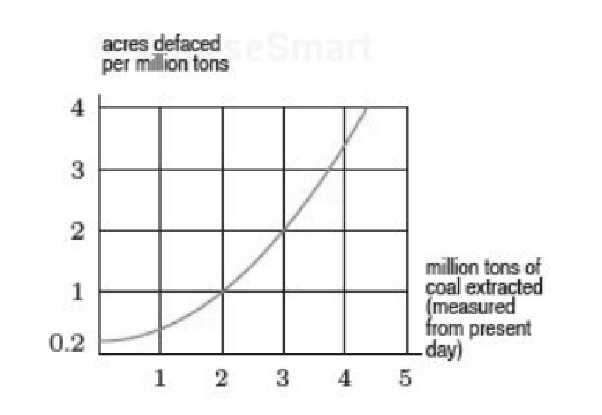
\includegraphics[width=0.8\linewidth]{graphics/Week04_DefiniteIntegralsInModeling/Coal}
  \end{Question}

  \begin{Solution}
    \begin{enumerate}[(a)]
\item ~\\
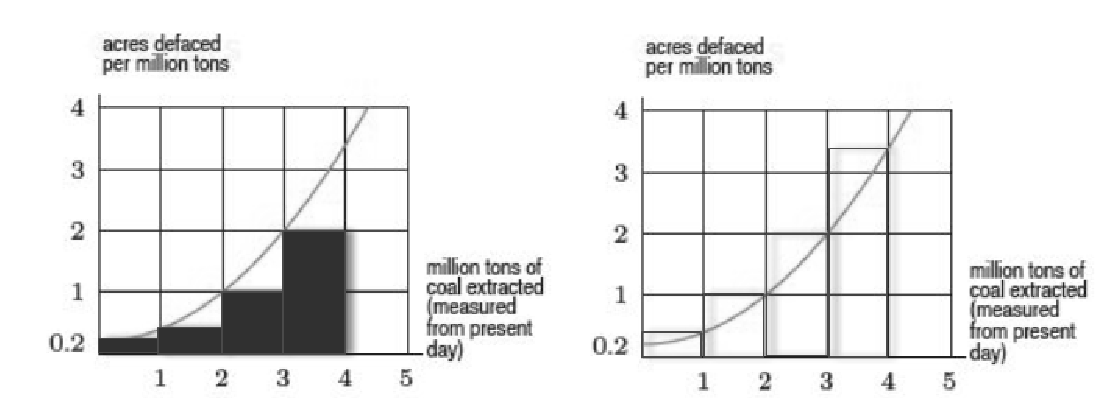
\includegraphics[width=1.0\linewidth]{graphics/Week04_DefiniteIntegralsInModeling/Coal_solutions} \\
Using rectangles under the curve, we get
$$\mbox{Acres defaced} \approx (1)(0.2 + 0.4 + 1 + 2) = 3.6 \mbox{ acres.}$$
\item Using rectangles above the curve, we get
$$\mbox{Acres defaced} \approx (1)(0.4 + 1 + 2 + 3.5) = 6.9 \mbox{ acres.}$$
\item The number of acres defaced is between 3.6 and 6.9, so we
  estimate the average, 5.25 acres.
    \end{enumerate}
  \end{Solution}


%*****************
\item
  \begin{Question}
    The following table gives the emissions, $E$, of nitrogen oxides,
    in millions of metric tons per year, in the US. Let $t$ be the
    number of years since 1970 and $E = f(t)$.
  \begin{enumerate}[(a)]
  \item  What are the units and meaning of $\ds \int^{30}_0 f(t)~dt$? 
\item Estimate $\ds \int^{30}_0 f(t)~dt$. 

\hspace{-0.5in}\begin{tabular}{lrrrrrrr} \hline
Year&1970&1975&1980&1985&1990&1995&2000\\ \hline
E&26.9&26.4&27.1&25.8&25.5&25.0&22.6  \\ \hline
\end{tabular}
  \end{enumerate}
  \end{Question}

  \begin{Solution}
    \begin{enumerate}[(a)]
    \item The integral $\ds \int^{30}_0 f(t)~dt$ represents the total
      emissions of nitrogen oxides, in millions of metric tons, during
      the period 1970 to 2000.
\item We estimate the integral using left- and right-hand sums:
\hspace{-0.5in}  \begin{align*}
\mbox{Left sum} &= (26.9)5 + (26.4)5 + (27.1)5 + (25.8)5 \\ & + (25.5)5 + (25.0)5 \\ &
= 783.5. \\
\mbox{Right sum} &= (26.4)5 + (27.1)5 + (25.8)5 + (25.5)5 \\ &+ (25.0)5 + (22.6)5 \\ &
= 762.0.\\
  \end{align*}
We average the left- and right-hand sums to find an improved estimate of the integral:
$$\int^{30}_ 0 f(t)~dt \approx \frac{783.5 + 762.0}{ 2} = 772.8 \mbox{ million metric tons.}$$
Between 1970 and 2000, about 772.8 million metric tons of nitrogen oxides were emitted.
    \end{enumerate}
  \end{Solution}

%*****************
\item
  \begin{Question}
Coal gas is produced at a gasworks. Pollutants in the gas are removed by scrubbers, which become less and less efficient as time goes on. The following measurements, made at the start of each month, show the rate at which pollutants are escaping (in tons/ month) in the gas: 
\begin{tabular}{lrrrrrrrr} \hline
Time (months)&0&1&2&3&4&5&6\\ \hline
 Rate pollutants escape&5&7&8&10&13&16&20 \\ 
(tons/month) & \\ \hline
\end{tabular} 
\begin{enumerate}[(a)]
\item Make an overestimate and an underestimate of the total quantity
  of pollutants that escape during the {\bf first month}.
\item Make an overestimate and an underestimate of the total quantity
  of pollutants that escape during the {\bf six months} shown in the table.
\end{enumerate}
  \end{Question}

  \begin{Solution}
    \begin{enumerate}[(a)]
    \item An overestimate is (7 tons/month)$\cdot$ (1 month) = 7 tons. An underestimate is (5 tons/month)$\cdot$(1 month) = 5 tons.
    \item An overestimate is 7+8+10+13+16+20 = 74 tons. An
      underestimate is 5+7+8+10+13+16 = 59 tons.
    \end{enumerate}
  \end{Solution}

%*****************
\item
  \begin{Question}
    The graph below shows the rate of change of the quantity of water
    in a water tower, in liters per day, during the month of April. If
    the tower had 12,000 liters of water in it on April 1, estimate
    the quantity of water in the tower on April 30.

\includegraphics[width=0.8\linewidth]{graphics/Week04_DefiniteIntegralsInModeling/WaterTower2}
  \end{Question}

  \begin{Solution}
    Suppose $V(t)$ represents the total quantity of water in the water
    tower at time $t$, where $t$ is in days since April 1. Then the
    graph shown in the problem is a graph of the volume's rate of
    change, or $\ddt{V}$ or $V'(t)$. By the Fundamental Theorem, the
    change in the volume over the 30 days of April is given by:
$$V(30) - V(0) = \int^{30}_0 V'(t)~dt.$$
This relationship means we can calculate the change in the volume of
water by calculating the area under the curve. Each box represents
about (50 l/d)$\cdot$(6 d) = 300 liters. 

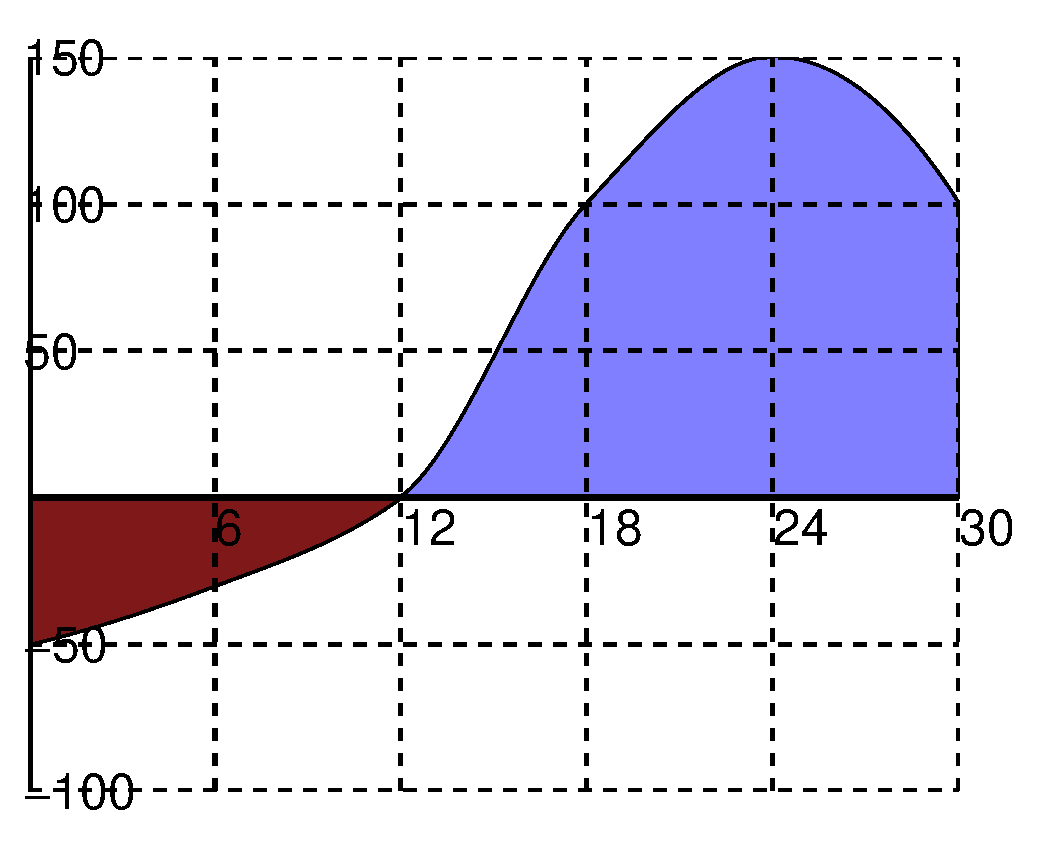
\includegraphics[width=0.8\linewidth]{graphics/Week04_DefiniteIntegralsInModeling/WaterTower2_soln}

In the red region, from $t = 0$ to $t = 12$, the graph is below the
$t$ axis, indicating that water is being lost from the tower.  There
is a little more than one
box, but for simplicity we'll call it one square, so roughly $\approx 300$ liters were lost.  \\
From $t = 12$ to $t = 30$ (blue region), there are between 6 and 7
boxes in total
(let's say 6 for simplicity), or roughly +1800 liters. \\
Thus, $$\int^{30}_0 V'(t)~dt \approx 1800 - 300 = 1500$$ This is the
net {\em change} in the volume of water.  Solving for $V(30)$, the
{\em amount} of water on April 30th,
\begin{align*}
V(30) & = V(0) + \int^{30}_0 V'(t)~dt \\ 
& = 12,000 + 1500 = 13,500 \mbox{ liters.}
\end{align*}
  \end{Solution}

%*****************
\item
  \begin{Question}
    A bicyclist pedals along a straight road with velocity $v$ given
    in the graph below. She starts 5 miles from a lake; positive
    velocities take her away from the lake and negative velocities
    take her toward the lake. When is the cyclist farthest from the
    lake, and how far away is she then?

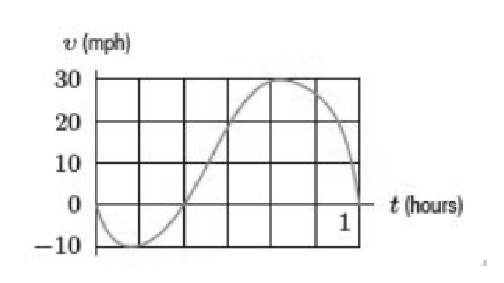
\includegraphics[width=0.8\linewidth]{graphics/Week04_DefiniteIntegralsInModeling/LakeCyclist}
  \end{Question}

  \begin{Solution}
    Notice that the area of a square on the graph represents (10 mph)$
    \cdot$ (1/6) h = (5/3) miles. 

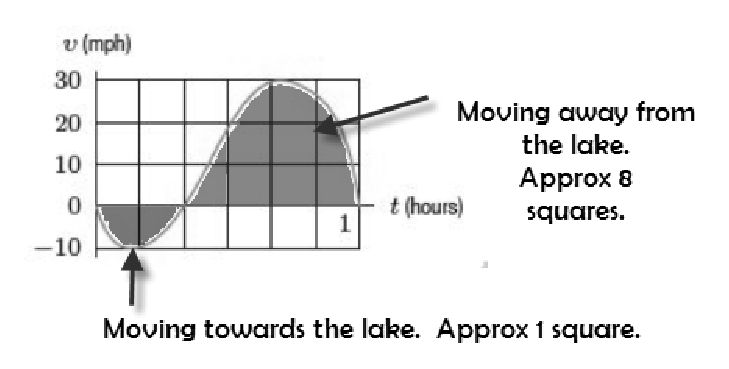
\includegraphics[width=1.0\linewidth]{graphics/Week04_DefiniteIntegralsInModeling/LakeCyclist_solutions}

At $t = 1/3$ hours, $v = 0$. The area between the curve $v$ and the
$t$-axis over the interval $0 \le t \le 1/3$ is $\ds -\int^{1/3}_0 v
~dt \approx \mbox{ one square} = 5/3$ miles.  Since $v$ is negative
here, she is moving toward the lake. Since she starts 5 miles from the
lake at time $t=0$, at $t = 1/3$ she is about 5 - 5/3 = 10/3 miles
from the lake (so closer than when she started).


For $1/3 \le t \le 1$, $v$ is positive, so she is moving away from the
lake.  Her {\em change} in distance from the lake between the times
$t=0$ and the end point $t=1$ is given by
\begin{align*}
\int^1_0 v ~dt & =
\int^{1/3}_0 v ~dt +
\int^1_{1/3} v ~dt \\
& \approx -
\frac{5}{3} + 8 \cdot
\frac{5}{3} =
\frac{35}{ 3} = 11.667 \mbox{ miles,}
\end{align*}
Relative to her starting point of 5 miles at $t=0$, the cyclist is
about 5 + 35/3 = 50/3 = 16.667 miles from the lake at $t=1$.  Since,
starting from the moment $t = 1/3$, she is always moving away from the
lake, the cyclist will be farthest from the lake at the latest
possible time, $t = 1$. The maximal distance at that time equals 50/3
= 16.667 miles.
  \end{Solution}

%*****************
\item
  \begin{Question}
    Height velocity graphs are used by endocrinologists (doctors
    specializing in the study of hormones) to follow the progress of
    children with growth deficiencies. The graph below shows the
    height velocity curves of an average boy and an average girl
    between ages 3 and 18.


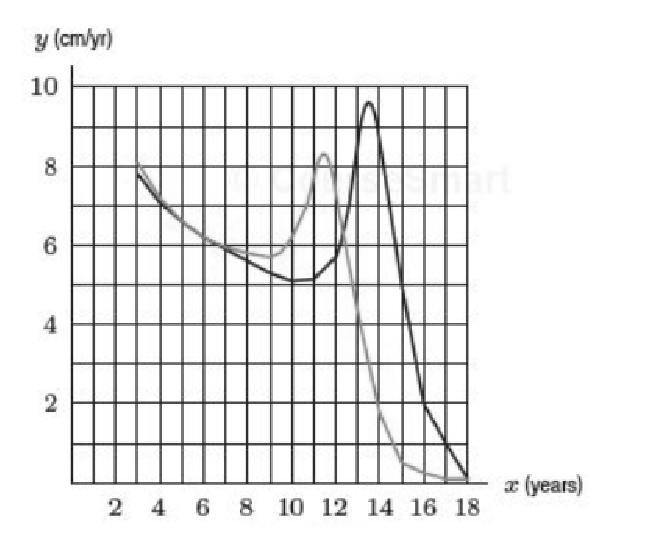
\includegraphics[width=0.8\linewidth]{graphics/Week04_DefiniteIntegralsInModeling/HeightVelocity}
\begin{enumerate}[(a)]
\item Which curve is for girls and which is for boys?  Explain how
  you can tell.
\item About how much does the average boy grow between ages 3 and
    10?
  \item The growth spurt associated with adolescence and the onset of
    puberty occurs between ages 12 and 15 for the average boy and
    between ages 10 and 12.5 for the average girl. Estimate the height
    gained by each average child during this growth spurt.
  \item When fully grown, about how much taller is the average man
    than the average woman? (The average boy and girl are about the
    same height at age 3.)
\end{enumerate}

  \end{Question}

  \begin{Solution}
    \begin{enumerate}[(a)]
    \item Since men are generally taller than women, the curve with
      the larger area under it is the height velocity of the boys.
      The area under each curve represents the change in growth in
      centimeters.  Therefore, the black curve is for boys, the
      lighter grey one for girls.
    \item Each square below the height velocity curve has area (1 cm/yr) $\cdot$
       1 yr = 1 cm. Counting squares lying below the black curve
      gives about 43 cm. Thus, on average, boys grow about 43 cm
      between ages 3 and 10.
    \item Counting squares lying below the black curve gives about 23
      cm growth for boys during their growth spurt. Counting squares
      lying below the colored curve gives about 18 cm for girls during
      their growth spurt.
    \item We can measure the difference in growth by counting squares
      that lie between the two curves. Between ages 2 and 12.5, the
      average girl grows faster than the average boy. Counting squares
      yields about 5 cm between the colored and black curves for $2 \le
      x \le 12.5$. Counting squares between the curves for $12.5 \le x \le
      18$ gives about 18 squares.  Thus, there is a net increase of
      boys over girls by about 18 - 5 = 13 cm.
    \end{enumerate}
  \end{Solution}

\end{multicols}

\hrulefill

\subsection*{Properties of Definite Integrals}

\begin{multicols}{2}
%*****************
\begin{Question}
\item[~] For questions \ref{q:even_odd_start} to \ref{q:even_odd_end} , find $\ds \int_2^5 f(x)~dx$.
\end{Question}
\item \label{q:even_odd_start}
  \begin{Question}
   $f(x)$ is odd and $\ds \int_{-2}^5 f(x)~dx = 8$.
  \end{Question}

  \begin{Solution}
    To use the fact that $f$ is odd, we split the interval up into the
    symmetric interval, [-2, 2], and the non-symmetric interval, [2,
    5].

    We have
 $$ 8 = \int_{-2}^5 \ifd = \int_{-2}^2 \ifd + \int_2^5 \ifd$$
 Since $f$ is odd, $\ds \int_{-2}^2 \ifd = 0$, so $\ds \int_{-2}^5
 \ifd = 8$.
  \end{Solution}
%*****************
\item
  \begin{Question}
   $f(x)$ is even, $\ds \int_{-2}^2 f(x)~dx = 6$, and $\ds \int_{-5}^5 f(x)~dx = 14$.
  \end{Question}

  \begin{Solution}
    Since $f$ is even,$ \ds \int_0^2 \ifd = (1/2) \cdot 6 = 3$  and $\ds \int_0^5
f(x)~dx = (1/2)\cdot 14 = 7$.\\
 Therefore
\begin{align*}
\int_2^5 f(x)~dx & = \int_0^5
f(x)~dx- \int_0^2 f(x)~dx \\
& = 7 - 3 = 4.
\end{align*}
  \end{Solution}
%*****************
\item
  \begin{Question}
   $\ds \int_2^5 (3 f(x) + 4)~dx) = 18.$ 
  \end{Question}

  \begin{Solution}
    We have
\begin{align*}
18 & = \int_2^5 (3f(x) + 4)~dx \\
& = 3 \int_2^5 f(x)~dx + \int_2^5 4~dx \\
\end{align*}
Thus, since $\ds \int_2^5 4~dx = 4(5-2) = 12$,  we have
$$3 \int_2^5 f(x)~dx = 18 - \underbrace{\int_2^5 4~dx}_{12} = 6$$
so $$\ds \int_2^5 f(x)~dx = \frac{6}{3} = 2.$$
  \end{Solution}
%*****************
\item\label{q:even_odd_end}
  \begin{Question}
   $\ds\int_2^4 2f(x)~dx = 8$ and $\ds \int_5^4 f(x)~dx = 1$. 
  \end{Question}

  \begin{Solution}
    We have
$\ds \int_2^4 f(x)~dx = 8/2 = 4$ and $\ds \int_4^5 f(x)~dx = - \int_5^4 f(x)~dx = -1$. Thus
\begin{align*}
\int_2^5 f(x)~dx & = \int^4_2 f(x)~dx +
\int^5_4 f(x)~dx\\ & = 4 - 1 = 3
\end{align*}
  \end{Solution}
%*****************
\item
  \begin{Question}
   Without any computation, find the values of
   \begin{enumerate}[(a)]
   \item $\ds \int_{-2}^2 \sin x~dx$. 
   \item $\ds \int_{-\pi}^\pi x^{113}~dx$.
   \end{enumerate}
  \end{Question}

  \begin{Solution}
    \begin{enumerate}[(a)]
    \item  0, since the integrand is an odd function and the limits are symmetric around 0. \\
\item 0, since the integrand is an odd function and the limits are symmetric around 0.   
    \end{enumerate}
  \end{Solution}
%*****************
\item
  \begin{Question}
    Without integrating, show that $$2 \le \ds \int_0^2 \sqrt{1 + x^3}
    ~dx \le 6.$$
  \end{Question}

  \begin{Solution}
    Notice that $f(x) = \sqrt{1 + x^3}$ is increasing for $0 \le x \le
    2$, since $x^3$ gets bigger as $x$ increases. This means that,
    looking at the interval [0, 2] over which we are integrating,
    $f(0) \le f(x) \le f(2)$. 


For this function, $f(0) = \sqrt{1 +0} = 1$ and $f(2) = \sqrt{1 + 8} = 3$. Thus, the area under
$f(x)$ lies between the area under the line $y = 1$ and the area under
the line $y = 3$ on the interval $0 \le x \le 2$. See the diagram
below.  

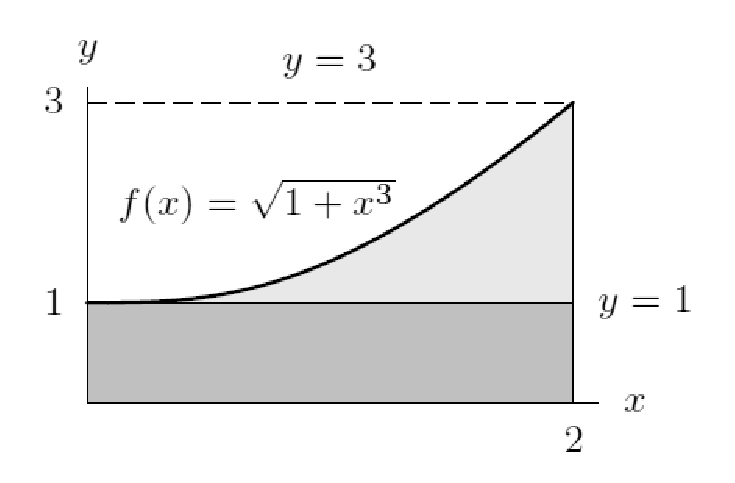
\includegraphics[width=0.8\linewidth]{graphics/Week04_PropertiesOfDefiniteIntegrals/IntegralBound1_solutions}

That is,
$$\underbrace{1}_h\underbrace{(2 - 0)}_w \le \int^2_0 \sqrt{ 1 + x^3}~dx \le \underbrace{3}_h\underbrace{(2 - 0)}_w$$

  \end{Solution}
%*****************
\item
  \begin{Question}
   Without calculating  the integral, explain why the following statements are false.
   \begin{enumerate}[(a)]
   \item $\ds \int_{-2}^{-1} e^{x^2} ~dx = -3$ 
   \item $\ds \int_{-1}^{1} \left| \frac{\cos(x+2)}{1 + \tan^2x} \right| ~dx = 0$.
   \end{enumerate}
  \end{Question}

  \begin{Solution}
    (a) The integrand is always positive, so the integral (sum of positive $f(x)$ times positive $\D x$ values) cannot be negative. \\
    (b) The integrand is always $\ge 0$ because of the absolute value
    sign. If the integral = 0, then with a non-negative integrand, the
    integrand must be exactly 0 at every $x$ value on the interval,
    which is definitely not the case here.
  \end{Solution}
%*****************
\item
  \begin{Question}
Based on the graph of $f(x)$ shown below, write $\ds \int_0^3 f(x)~dx$ in terms 
of $\ds \int_{-1}^1 f(x)~dx$ and $\ds \int_{1}^3 f(x)~dx$.

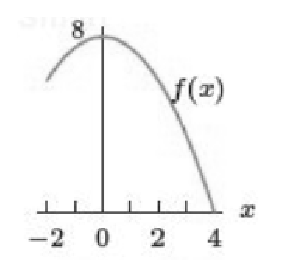
\includegraphics[width=0.4\linewidth]{graphics/Week04_PropertiesOfDefiniteIntegrals/EvenIntegral}
  \end{Question}

  \begin{Solution}
We know that we can divide the integral up as follows:
$$\ds \int^3_0 f(x)~dx = \int^1_0 f(x)~dx + \int^3_1 f(x)~dx.$$
The graph suggests that $f$ is an even function for $-1 \le x \le 1$, so
$\int^1_{-1} f(x)~dx = 2 \int^1_0 f(x)~dx$. Substituting this into
the preceding equation, we have
$$\int^3_0 f(x)~dx = \frac{1}{2} \int^1_{-1} f(x)~dx + \int^3_1 f(x)~dx.$$
    
  \end{Solution}
%*****************
\item
  \begin{Question}
    Using the graph of $f(x)$ shown below, arrange the following
    quantities in increasing order, from least to greatest.

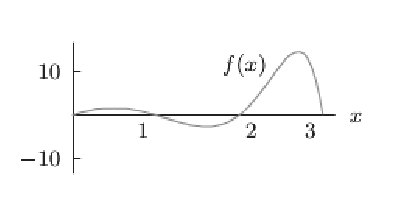
\includegraphics[width=0.6\linewidth]{graphics/Week04_PropertiesOfDefiniteIntegrals/IntegralRanking}

\begin{tabular}{ll}
(i) $\ds \int_0^1 f(x)~dx $ & 
(ii)$\ds \int_1^2  f(x)~dx $ \\
(iii)$\ds \int_0^2  f (x)~dx $ & 
(iv) $\ds \int_2^3 f(x)~dx $ \\
(v) $-\ds \int_1^2  f(x)~dx $ &
(vi) The number 0  \\
(vii) The number 20  &
(viii) The number -10
\end{tabular}
  \end{Question}

  \begin{Solution}
    See the figure below.

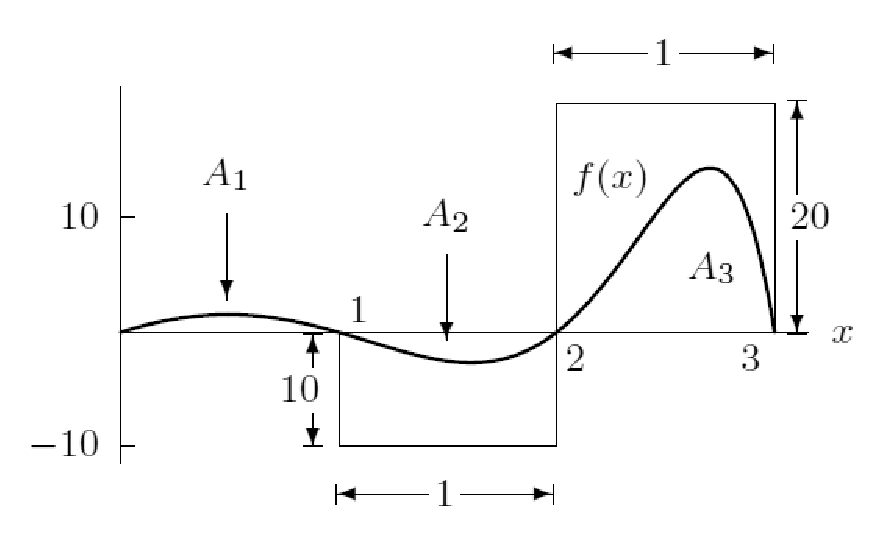
\includegraphics[width=0.8\linewidth]{graphics/Week04_PropertiesOfDefiniteIntegrals/IntegralRanking_solutions}

Since $\ds \int^1_0 f(x)~dx = A_1$ and
$\ds \int^2_1 f(x)~dx = -A_2$ and
$\ds \int^3_2 f(x)~dx = A_3$, we know that
$$0 < \int^1_0 f(x)~dx < - \int^2_1 f(x)~dx < \int^3_2 f(x)~dx.$$
In addition,
$\ds \int^2_0 f(x)~dx = A_1 - A_2$, which is negative, but smaller in magnitude than
$\ds \int^2_1 f(x)~dx$. Thus
$$\int^2_1 f(x)~dx < \int^2_0 f(x)~dx < 0.$$
The area $A_3$ lies inside a rectangle of height 20 and base 1, so
$A_3 < 20$.   \\
The area $A_2$ lies inside a rectangle below the $x$-axis of
height 10 and width 1, so $-10 < A_2$. Thus: 
\begin{center}
(viii) $<$ (ii) $<$ (iii) $<$ (vi) $<$ (i) $<$ (v) $<$ (iv) $<$ (vii).
\end{center}
  \end{Solution}
%*****************
\item
  \begin{Question}
    \begin{enumerate}[(a)]
    \item Use the graph of $y = x e^{-x^2}$ shown below to explain why $\ds \int_{-3}^3 x e^{-x^2} ~dx= 0$.
\begin{center}
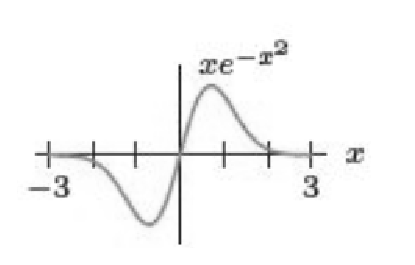
\includegraphics[width=0.5\linewidth]{graphics/Week04_PropertiesOfDefiniteIntegrals/xexp_integral}
\end{center}

    \item Find the left-hand sum approximation with $n = 3$ to $\ds
      \int_{0}^3 x e^{-x^2}~dx$. Give your answer to four decimal
      places.
    \item Repeat part (b) for $\ds \int_{-3}^0 x e^{-x^2}~dx$.
    \item Do your answers to parts (b) and (c) add to 0? Explain.
    \end{enumerate}
  \end{Question}

  \begin{Solution}
    \begin{enumerate}[(a)]
    \item Since the function is odd, and the interval used is
      symmetric across $x=0$, the areas above and below the x-axis
      cancel. Thus,
$$\ds\int^0_{-3} xe^{-x^2} dx = -
\int^3_0 xe^{-x^2} dx,$$
 $$\mbox{ so } \ds \int^3_{-3} xe^{-x^2} dx =
\underbrace{\int^0_{-3} xe^{-x^2} dx +
\int^3_0 xe^{-x^2} dx}_{\mbox{equal magnitude, opposite signs}} = 0.$$
\item For $0 \le x \le 3$ with $n = 3$, we have $x_0 = 0, x_1 = 1, x_2 = 2, x_3 = 3$, and $\D x = 1$. See the figure below. 

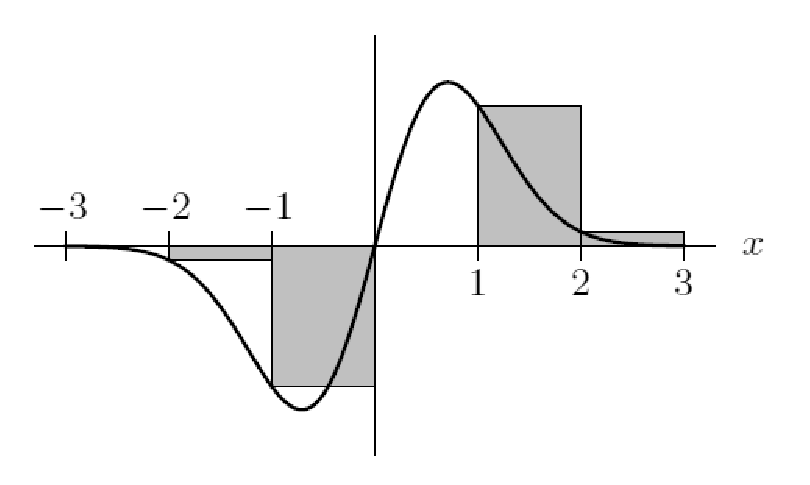
\includegraphics[width=0.8\linewidth]{graphics/Week04_PropertiesOfDefiniteIntegrals/xexp_integral_solutions}

\begin{align*}
\mbox{Left sum}& = f(x_0)\D x + f(x_1)\D x + f(x_2)\D x \\
& = 0e^{-0^2} \cdot 1 + 1e^{-(1^2)} \cdot 1 + 2e^{-(2^2)} \cdot 1 \\
& = 0.4045.
\end{align*}
\item For $-3 \le x \le 0$, with $n = 3$, we have $x_0 = -3, x_1 = -2, x_2 = -1, x_3 = 0$, and $\D x = 1$. (See the diagram again.)
\begin{align*}
\mbox{Left sum} & = f(x_0)\D x + f(x_1)\D x + f(x_2)\D x \\
& = -3e^{-(-3)^2}
\cdot 1 - 2e^{-(-2)^2}
\cdot 1 - 1e^{-(-1)^2}
\cdot 1 \\
& = -0.4049. \\
\end{align*}
\item No. The rectangles between $x=-3$ and 0 are not the same size as
  those between $x=0$ and 3. See the diagram.  There are three
  rectangles with nonzero height on [-3, 0] and only two on [0, 3], so
  the estimates computed must be different, so we won't get the exact
  result of zero using left sums.
    \end{enumerate}
  \end{Solution}

\end{multicols}
\hrulefill

\subsection*{Integration By Anti-Derivatives}

\begin{Question}
  To practice computing anti-derivatives, do as many of the
  problems from the following section as you need.
\end{Question}

\begin{multicols}{2}

From Hughes-Hallett 5th edition,  \\
Section 6.2 - 1-63 (odd)
\columnbreak

From Hughes-Hallett 6th edition,  \\
Section 6.2 - 1-60 (odd)

\end{multicols}
Note: In questions 53-63 (5th Ed.) and 51-60 (6th Ed.), `evaluate
numerically'  means `plug the limit values into the anti-derivative
using your calculator to get a decimal number'. It does {\em not} mean
use rectangles/trapezoids/Riemann sums to approximate the integral
values.  

\hrulefill

Additional problems. Evaluate the following integrals.

\item \begin{Question}
  $\ds \int_{-1}^2 (x^3 - 2x) dx$
\end{Question}

\begin{Solution}
  $\ds \int_{-1}^2 (x^3 - 2x) dx = \left[ \frac{x^4}{4} - x^2 
    \right]_{-1}^2 = \left( \frac{2^4}{4} - 2^2 \right) - \left( \
      \frac{(-1)^4}{4} - (-1)^2 \right) = (4 - 4) - (\frac{1}{4} - 1) = 0
    - (- \frac{3}{4}) = \frac{3}{4}$
\end{Solution}

\item \begin{Question}
  $\ds \int_{-1}^1 x^{100} dx$
\end{Question}

\begin{Solution}
  $\ds \int_{-1}^1 x^{100} dx = \left[ \frac{1}{101} x^{101} 
    \right]_{-1}^{1} = \frac{1}{101} - (- \frac{1}{101}) = 
    \frac{2}{101}$
\end{Solution}

\item \begin{Question}
  $\ds \int_{1}^4 (5 - 2t +3t^2) dt$
\end{Question}

\begin{Solution}
  $\ds \int_1^4 (5 - 2t - 3t^2) dt = [5t - t^2 + t^3]_1^4 = 
    (20 - 16 + 64) - (5 - 1 + 1) = 68 - 5 = 63$
\end{Solution}

\item \begin{Question}
  $\ds \int_0^1 (1 + \frac{1}{2} u^4 - \frac{2}{5} u^9) du$
\end{Question}

\begin{Solution}
  $\int_0^1 (1 + \frac{1}{2} u^4 - \frac{2}{5} u^9) du = 
    [u + \frac{1}{10} u^5 - \frac{1}{25} u^10]_0^1 = 
    (1 + \frac{1}{10} - \frac{1}{25}) - 0 = \frac{50 + 5 - 2}{50} = \frac{53}{50}$
\end{Solution}

\item \begin{Question}
  $\ds \int_1^9 \sqrt{x} dx$
\end{Question}

\begin{Solution}
  $\ds \int_1^9 \sqrt{x} dx = \int_1^9 x^{1 / 2} dx = 
    \left[ \frac{x^{3 / 2}}{3 / 2} \right]_1^9 =
    \frac{2}{3} \left[ x^{2 / 3} \right]_1^9 =
    \frac{2}{3} (9^{3 / 2} - 1^{3 / 2}) = 
    \frac{2}{3} (27 - 1) = \frac{52}{3}$
\end{Solution}

\item \begin{Question}
    
  $\ds \int_1^8 x^{-2 / 3} dx$
\end{Question}

\begin{Solution}
    
  $\ds \int_1^8 x^{-2 / 3} dx = 
    \left[ \frac{x^{1 / 3}}{1 / 3} \right]_1^8 = 
    3 \left[ x^{1 / 3} \right]_1^8 = 
    3(8^{1 / 3} - 1^{1 / 3}) = 3(2 - 1) = 3$
    
\end{Solution}

\item \begin{Question}
    
  $\ds \int_{\pi / 6}^{\pi} \sin \theta d \theta$
\end{Question}

\begin{Solution}
  $\ds \int_{\pi / 6}^{\pi} \sin \theta d \theta =
    \left[ - \cos \theta \right]_{\pi / 6}^{\pi} =
    - \cos \pi - ( - \cos \frac{\pi}{6} ) = 
    -(-1) - (- \sqrt{3} / 2) = 1 + \sqrt{3} / 2$
\end{Solution}

\item \begin{Question}
    
  $\ds \int_{-5}^5 e~ dx$
\end{Question}

\begin{Solution}
  The number $e$ is just a constant. 

    $\ds \int_{-5}^5 e ~dx = [e x]_{-5}^5 = 5e - (-5e) = 10e$
    
\end{Solution}

\item \begin{Question}
    
  $\ds \int_0^1 (u + 2)(u - 3) du$
\end{Question}

\begin{Solution}
  You need to expand the product before you can integrate.  

    $\ds \int_0^1 (u + 2)(u - 3) du = \int_0^1 (u^2 - u - 6) du = \left[
      \frac{1}{3} u^3 - \frac{1}{2} u^2 - 6u \right]_0^1 =
    \left(\frac{1}{3} - \frac{1}{2} - 6 \right) - 0 = - \frac{37}{6}$
\end{Solution}


  \item \begin{Question}
  $\ds \int_0^4 (4 - t) \sqrt{t} ~dt$
\end{Question}

\begin{Solution}
To evaluate this integral, you need to expand the product first; you can't integrate the product $(4-t)\sqrt{t}$ as it is originally written.

  $\ds \int_0^4 (4 - t) \sqrt{t} dt = \int_0^4 (4 - t) t^{1 / 2} dt =
    \int_0^4 (4t^{1 / 2} - t^{3 / 2}) dt = 
    \left[ \frac{8}{3} t^{3 / 2} - \frac{2}{5} t^{5 / 2} \right]_0^4 =
    \frac{8}{3} (8) - \frac{2}{5} (32) = 
    \frac{320 - 192}{15} = \frac{128}{15}$
\end{Solution}

\item \begin{Question}
    
  $\ds \int_1^9 \frac{x - 1}{\sqrt{x}} dx$
\end{Question}

\begin{Solution}
    
  $\ds \int_1^9 \frac{x - 1}{\sqrt{x}} dx =
    \int_1^9 \left( \frac{x}{\sqrt{x}} - \frac{1}{\sqrt{x}} \right) dx
    = \int_1^9 (x^{1 / 2} - x^{-1 / 2}) dx =
    \left[\frac{2}{3} x^{3 / 2} - 2x^{1 / 2} \right]_1^9 = 
    (\frac{2}{3} \cdot 27 - 2 \cdot 3) = (\frac{2}{3} - 2) = 
    12 - (- \frac{4}{3}) = \frac{40}{3}$
\end{Solution}

\item \begin{Question}
    
  $\ds \int_0^2 (y - 1)(2y + 1) dy$
\end{Question}

\begin{Solution}
    
  $\ds \int_0^2 (y - 1)(2y + 1) dy = \int_0^2 (2y^2 - y - 1) dy =
    \left[ \frac{2}{3} y^3 - \frac{1}{2} y^2 - y \right]_0^2 = 
    ( \frac{16}{3} - 2 - 2) - 0 = \frac{4}{3}$
\end{Solution}

\item \begin{Question}
    
  $\ds \int_0^{\pi / 4} \sec^2 t ~dt$
\end{Question}

\begin{Solution}
    
  $\ds \int_0^{\pi / 4} \sec^2 t ~dt = [\tan t]_0^{\pi / 4} =
    \tan \frac{\pi}{4} - \tan 0 = 1 - 0 = 1$
    
\end{Solution}

\item \begin{Question}
    
  $\ds \int_0^{\pi / 4} \sec \theta \tan \theta d \theta$
\end{Question}

\begin{Solution}
  $\ds \int_0^{\pi / 4} \sec \theta \tan \theta d \theta = 
    [ \sec \theta ]_0^{\pi / 4} = 
    \sec \frac{\pi}{4} - \sec 0 = \sqrt{2} - 1$
\end{Solution}

\item \begin{Question}
    
  $\ds \int_1^2 (1 + 2y)^2 dy$
\end{Question}

\begin{Solution}
  $\ds \int_1^2 (1 + 2y)^2 dy = 
    \int_1^2 (1 + 4y + 4y^2) dy =
    [y + 2y^2 + \frac{4}{3} y^3]_1^2 =
    (2 + 8 + \frac{32}{3}) - (1 + 2 + \frac{4}{3}) = 
    \frac{62}{3} - \frac{13}{3} = \frac{49}{3}$
\end{Solution}

\item \begin{Question}
    
  $\ds \int_0^3 (2 \sin x - e^x) dx$
\end{Question}

\begin{Solution}
  $\ds \int_0^3 (2 \sin x - e^x) dx = 
    [-2 \cos 3 - e^3) - (-2 - 1) =
    3 - 2 \cos 3 - e^3$
    
\end{Solution}

\item \begin{Question}
    
  $\ds \int_1^2 \frac{v^3 + 3v^6}{v^4} dv$
\end{Question}

\begin{Solution}
  $\ds \int_1^2 \frac{v^3 + 3v^6}{v^4} =
    \int_1^2 \left( \frac{1}{v} + 3v^2 \right) dv =
    [ \ln |v| + v^3]_1^2 = 
    ( \ln 2 + 8 ) - ( \ln 1 + 1) =
    \ln 2 + 7$
\end{Solution}

\item \begin{Question}
    
  $\ds \int_1^{18} \sqrt{\frac{3}{z}} dz$
\end{Question}

\begin{Solution}
  $\ds \int_1^{18} \sqrt{\frac{3}{z}} dz =
    \int_1^{18} \sqrt{3} z^{-1/2} dz =
    \sqrt{3} [ 2z^{1/2} ]_1^{18} =
    2 \sqrt{3} (18^{1/2} - 1^{1/2}) = 
    2 \sqrt{3} (3 \sqrt{2} - 1)$
\end{Solution}

\item \begin{Question}
    
  $\ds \int_0^1 (x^e + e^x) dx$
\end{Question}

\begin{Solution}
    
  $\ds \int_0^1 (x^e e^x) dx = 
    \left[ \frac{x^{e + 1}}{e + 1} + e^x \right]_0^1 =
    \left( \frac{1}{e + 1} + e \right) - (0 + 1) = 
    \frac{1}{e + 1} + e - 1$
\end{Solution}

\item \begin{Question}
    
  $\ds \int_{1 / \sqrt{3}}^{\sqrt{3}} \frac{8}{1 + x^2} dx$
\end{Question}

\begin{Solution}
  $\ds \int_{1 / \sqrt{3}}^{\sqrt{3}} \frac{8}{1 + x^2} dx =
    \left[ 8 \arctan x \right]_{1 / \sqrt{3}}^{\sqrt{3}} =
    8 \left( \frac{\pi}{3} - \frac{\pi}{6} \right) =
    8 \left( \frac{\pi}{6} \right) = \frac{4 \pi}{3}$
    
\end{Solution}

\item \begin{Question}
    
  $\ds \int_1^2 \frac{4 + u^2}{u^3} du$
\end{Question}

\begin{Solution}
  $\ds \int_1^2 \frac{4 + u^2}{u^3} du =
    \int_1^2 (4u^{-3} + u^{-1}) du =
    \left[ \frac{4}{-2} u^{-2} + \ln |u| \right]_1^2 =
    \left[ \frac{-2}{u^2} + \ln u \right]_1^2 =
    (-\frac{1}{2} + \ln 2) - (-2 + \ln 1) = 
    \frac{3}{2} + \ln 2$
\end{Solution}

\item \begin{Question}
    
  $\ds \int_{-1}^1 e^{u + 1} du$
\end{Question}

\begin{Solution}
  $\ds \int_{-1}^1 e^{u + 1} du = 
    [e^{u + 1}]_{-1}^1 =
    e^2 - e^0 = e^2 - 1$ [or start with $e^{u + 1} = e^u e^1$]
\end{Solution}

\item \begin{Question}
    
  $\ds \int_{1 / 2}^{1 / \sqrt{2}} \frac{4}{\sqrt{1 - x^2}} dx$
\end{Question}

\begin{Solution}
  $\ds \int_{1/2}^{1 / \sqrt{2}} \frac{4}{\sqrt{1 - x^2}} dx =
    \left[ 4 \arcsin x \right]_{1/2}^{1 / \sqrt{2}} =
    4 \left( \frac{\pi}{4} - \frac{\pi}{6} \right) =
    4(\frac{\pi}{12}) = \frac{\pi}{3}$
\end{Solution}

\item \begin{Question}
    
$\ds    \int_0^{\pi} f(x) dx \text{ where } f(x) = 
    \begin{cases}
      \sin x  & \text{ if } 0 \leq x < \pi / 2 \\
      \cos x  & \text{ if } \pi / 2 \leq x \leq \pi \\
    \end{cases}
   $ 

\end{Question}

\begin{Solution}
  $\ds \text{If } f(x) = 
    \begin{cases}
      \sin x  & \text{ if } 0 \leq x < \pi / 2 \\
      \cos x  & \text{ if } \pi / 2 \leq x \leq \pi \\
    \end{cases}
    $ then
    
    $\ds \int_{0}^{\pi} f(x) dx = 
    \int_0^{\pi/2} \sin x dx + \int_{\pi/2}^{\pi} \cos x dx =
    [ - \cos x]_0^{\pi/2} + [ \sin x ]_{\pi / 2}^{\pi} =
    - \cos \frac{\pi}{2} + \cos 0 + \sin \pi - \sin \frac{\pi}{2} = 
    -0 + 1 + 0 - 1 = 0$
\end{Solution}

\item \begin{Question}
    
$\ds    \int_{-2}^2 f(x) dx \text{ where } f(x) = 
    \begin{cases}
      2  & \text{ if } -2 \leq x \leq 0 \\
      4 - x^2 & \text{ if } 0 < x \leq 2 \\
    \end{cases}
  $ 
\end{Question}

\begin{Solution}
  $\ds \text{If } f(x) =
    \begin{cases}
      2  & \text{ if } -2 \leq x \leq 0 \\
      4 - x^2 & \text{ if } 0 < x \leq 2 \\
    \end{cases}
    $ then
    
    $\ds \int_{-2}^{2} f(x) dx =
    \int_{-2}^{0} 2 dx + \int_0^2 (4 - x^2) dx = 
    [2x]_{-2}^{0} + [4x - \frac{1}{3} x^3 ]_0^2 =
    [0 - (-4)] + (\frac{16}{3} - 0) = \frac{28}{3}$
    
\end{Solution}



\end{enumerate}
\end{document}

%*****************
\item
  \begin{Question}
    
  \end{Question}

  \begin{Solution}
    
  \end{Solution}
